% ====================================================================
% JAISP internal seminar deck -- Worsened astrometry: diagnosis and cure
% Build:  pdflatex worsened_astrometry.tex  (run twice; latexmk broken)
% Figures pulled from ../../io/_nb23_outputs, _nb24_outputs, _nb31_outputs, _nb32_outputs (copies in figures/)
% ====================================================================
\documentclass[aspectratio=169,10pt]{beamer}

\usepackage{graphicx}
\usepackage{booktabs}
\usepackage{amsmath,amssymb}
\usepackage{tikz}
% SUPERSEDED banner for the interim-mitigation (router) slides
\newcommand{\supersededbanner}{%
  \begin{tikzpicture}[remember picture,overlay]
    \node[anchor=north, yshift=-8.2mm, minimum width=\paperwidth, minimum height=4mm,
          fill=red!12, draw=none, inner sep=1.5pt]
      at (current page.north)
      {\scriptsize\bfseries\color{red!70!black}
       JULY 2026: INTERIM MITIGATION --- superseded by the v11 foundation fix (slides 13--18)};
  \end{tikzpicture}\vspace{1.4em}}
\graphicspath{{figures/}{../../io/_nb23_outputs/}{../../io/_nb24_outputs/}{../../io/_nb31_outputs/}{../../io/_nb32_outputs/}{../../paper/figures/}}

\usetheme{default}
\usecolortheme{seagull}
\setbeamertemplate{navigation symbols}{}
\setbeamertemplate{itemize items}[circle]
\setbeamertemplate{itemize subitem}[circle]

\definecolor{jaispblue}{RGB}{20,60,110}
\definecolor{jaispteal}{RGB}{0,120,130}
\definecolor{jaispaccent}{RGB}{190,70,25}
\setbeamercolor{frametitle}{fg=white,bg=jaispblue}
\setbeamercolor{title}{fg=jaispblue}
\setbeamercolor{structure}{fg=jaispblue}
\setbeamercolor{alerted text}{fg=jaispaccent}
\setbeamerfont{frametitle}{series=\bfseries,size=\large}
\setbeamertemplate{frametitle}{%
  \vspace*{0.25em}%
  \begin{beamercolorbox}[wd=\paperwidth,sep=0.5em]{frametitle}%
    \insertframetitle\hfill{\normalfont\small\insertframenumber/\inserttotalframenumber}%
  \end{beamercolorbox}}

% slightly smaller body fonts than the 10pt defaults (size9.clo unavailable)
\makeatletter
\renewcommand\normalsize{\@setfontsize\normalsize{9.3}{11.2}}
\renewcommand\small{\@setfontsize\small{8.6}{10.2}}
\renewcommand\footnotesize{\@setfontsize\footnotesize{8.0}{9.4}}
\makeatother

\newcommand{\jaisp}{\textsc{Jaisp}}
\newcommand{\mas}{\ensuremath{\,\mathrm{mas}}}

\title{Why Astrometry Is Degraded for a Subset of Objects:\\
  \Large Diagnosis and Cure in \jaisp{}}
\author{}
\institute{}
\date{July 2026, updated August and September 2026 \quad (internal, ECDFS Q1)}

\begin{document}

\begin{frame}[plain]
  \titlepage
\end{frame}

% --------------------------------------------------------------
\begin{frame}{The mystery: sources above the 1:1 line}
  \begin{columns}
    \column{0.46\textwidth}
      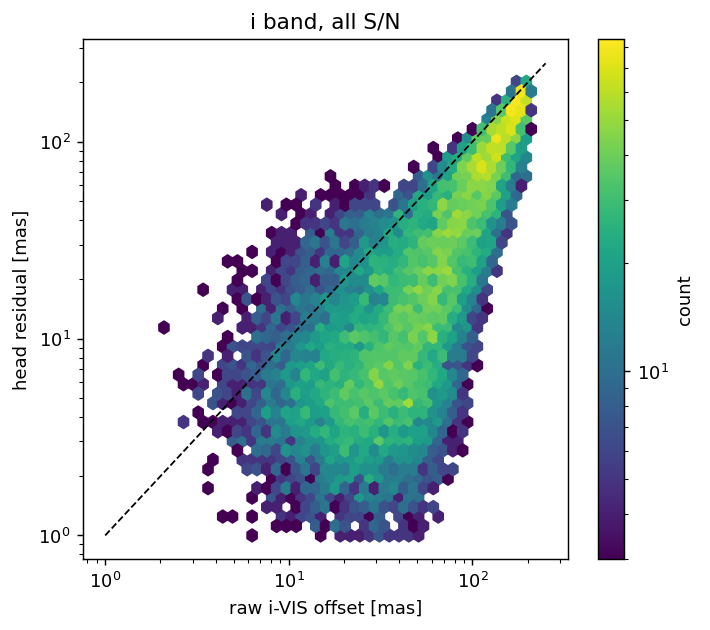
\includegraphics[width=\textwidth]{worseners_panel1.png}
    \column{0.52\textwidth}
      \begin{itemize}
        \item The head (\alert{v10 production}) improves the population (raw $\sim$48\mas{} $\to$ 13.4\mas{} median, all bands; panel: i band), but 9\% of all measurements end up \alert{farther} from VIS than they started.
        \item Two candidate explanations: (a) those sources were lucky before, and the small raw offset was chance; (b) the model fails on those sources specifically.
      \end{itemize}
  \end{columns}
\end{frame}

% --------------------------------------------------------------
\begin{frame}{Most of it is chance: regression to the corrected floor}
  \begin{center}
    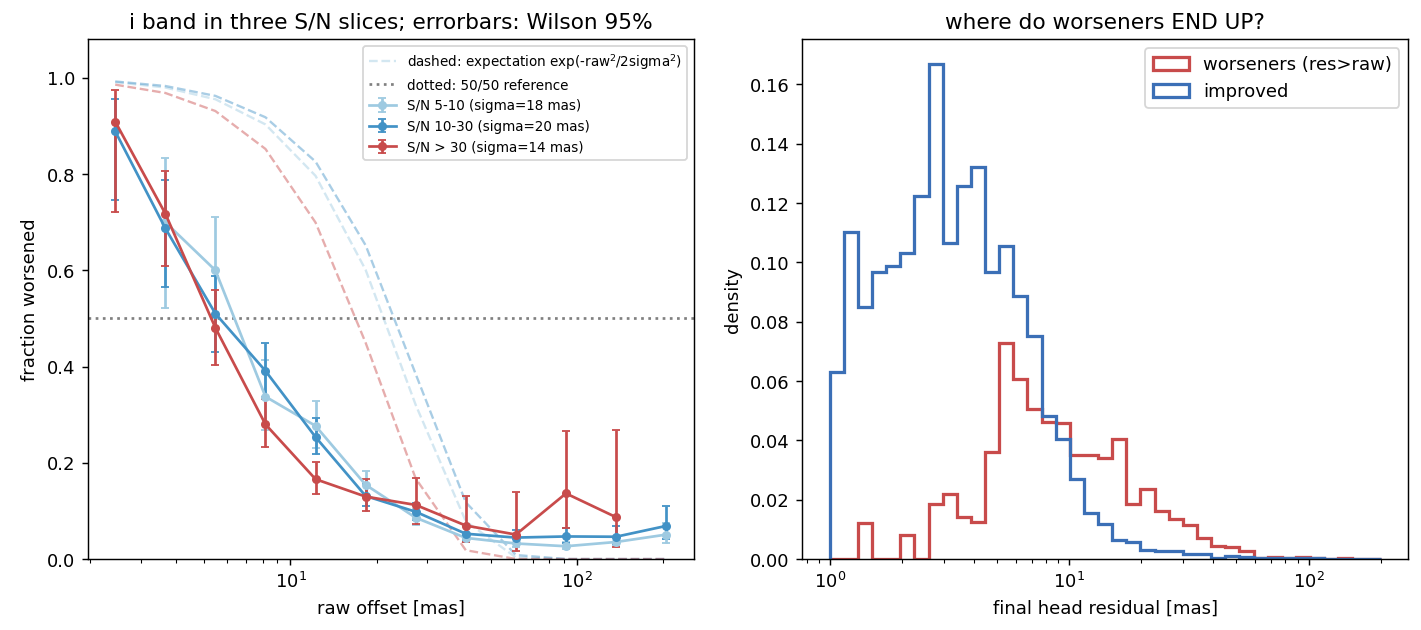
\includegraphics[width=0.78\textwidth]{worseners_panels23.png}\\{\scriptsize v10 production head}
  \end{center}
  \vspace{-0.5em}
  {\small
  \begin{itemize}
    \item Left: the same pattern in every S/N slice, each observed curve below its own re-measurement expectation (dashed, $P(\mathrm{worse})=e^{-\mathrm{raw}^2/2\sigma^2}$); pooled over bands, shared photons preserve lucky agreement more often than chance predicts.
    \item Only the \alert{bright} slice grows a tail at large raw offsets, where chance predicts zero. Right: worseners sit right of the improved because the selection forces it (res $>$ raw truncates the floor distribution from below); the truncated-floor prediction is 21.6\mas{} median versus 17.8 observed. Only the excess beyond ${\sim}40$\mas{} escapes any chance model.
  \end{itemize}}
\end{frame}

% --------------------------------------------------------------
\begin{frame}{Flash-forward: the same panel under v11 --- and why it hides the disease}
  \begin{center}
    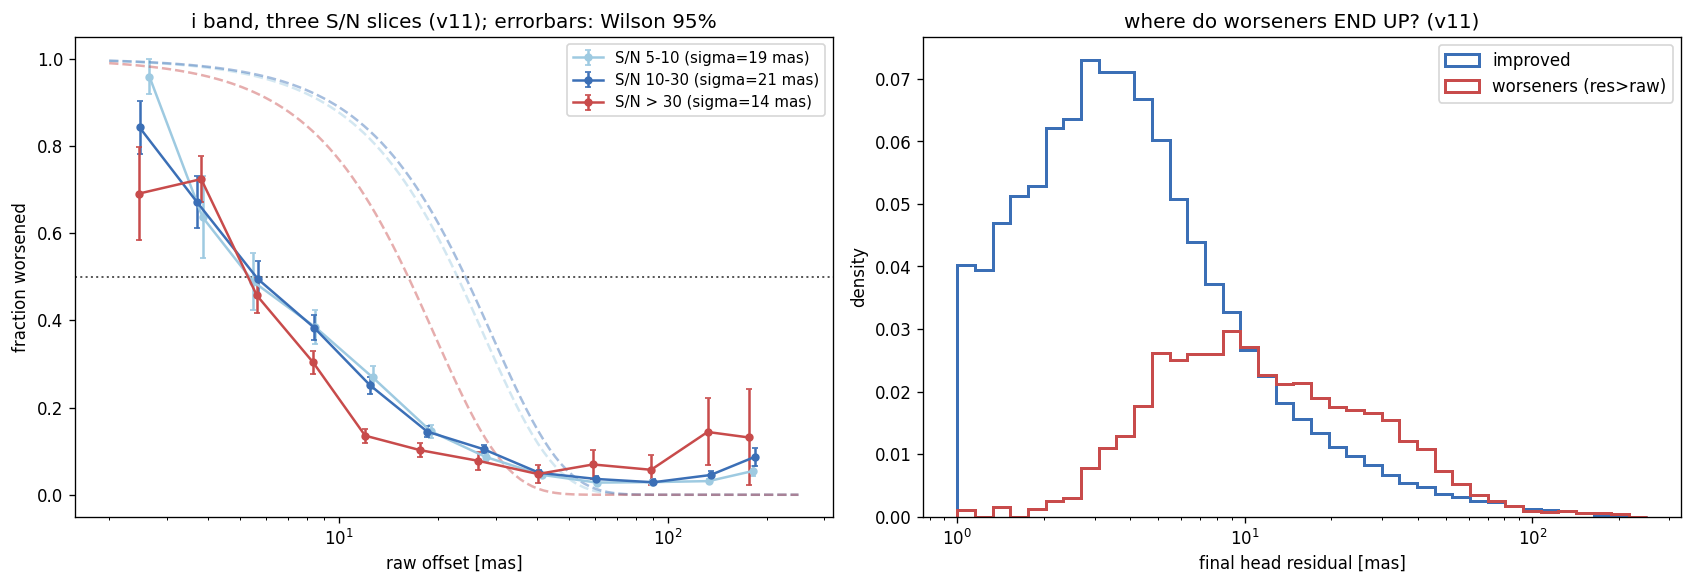
\includegraphics[width=0.74\textwidth]{worseners_panels23_v11.png}
  \end{center}
  \vspace{-0.5em}
  {\footnotesize
  \begin{itemize}
    \item After the fix (v11, slides ahead) this projection looks \alert{nearly identical} --- because the S/N$>$30 slice \alert{dilutes} the clamped stars (S/N$\gtrsim$100) with many unclamped ones. Cut the same plot at \alert{S/N$>$100}, raw 10--16\mas{} --- exactly where the affected stars live --- and the fix is dramatic: worsened \alert{48\% $\to$ 11\%}.
    \item The tail beyond raw $\sim$60\mas{} that escapes chance is \alert{neither} the clamp population \alert{nor} the later survivors (both live at small raw): it is 9 isolated $k{=}0$ large-amplitude flukes (res $\sim$100\mas{} in \emph{both} versions; likely matching/blend errors).
    \item Lesson: marginal projections have wildly different sensitivity to the same population --- which is why the next slide counts \alert{repetition across bands} instead.
  \end{itemize}}
\end{frame}

% --------------------------------------------------------------
\begin{frame}{Can repetition across bands be chance? Setting up the bookkeeping}
  \small
  For one source, per band $b$: fit the classical centroid, form $\mathrm{raw}_b = \mathrm{pos}_b - \mathrm{pos}_{\rm VIS}$; the head (v10) predicts a correction $c_b$ from one shared representation; $\mathrm{resid}_b = \mathrm{raw}_b - c_b$. ``Strongly worsened in $b$'' $=$ $|\mathrm{resid}_b| > 1.5\,|\mathrm{raw}_b|$ and worse by $>10$\mas. Rate: 5.6\% of bright measurements.
  \vspace{0.4em}
  \begin{itemize}
    \item \textbf{Independent between bands:} the centroid-fit noise of each band image (different exposures, different photons). If this alone drove worsening, hits on the same source would be independent coin flips: $P(3\ \mathrm{hits}) \approx 0.056^3 \times 10\ \mathrm{triples} \times 3185\ \mathrm{sources} \approx 5$.
    \item \textbf{Shared for one source:} (1) the VIS reference position, subtracted from every band; (2) the local WCS terms (Rubin bands share Rubin's solution, NISP its own); (3) the source itself (proper motion, colour gradients); (4) the head's shared representation, feeding all nine corrections.
  \end{itemize}
  \vspace{0.2em}
  \begin{center}
  \begin{tabular}{lcc}
    \toprule
    strongly worsened in $\geq k$ Rubin bands & observed & chance (permutation null) \\
    \midrule
    $k\geq2$ & 181 & $68\pm7$ \\
    $k\geq3$ & 113 & $5\pm2$ \\
    $k\geq4$ & 61 & $0.2$ \\
    $k\geq5$ & 23 & $0.0$ \\
    \bottomrule
  \end{tabular}
  \end{center}
  \vspace{0.2em}
  {\footnotesize The null shuffles flags within (band, raw offset, S/N) classes, preserving all rates and the VIS-induced raw correlations (hence chance $k\geq2$ is 68, not 0). Robust to the cuts (S/N$>$10: 200 vs 8; all nine bands: 153 vs 12) and to the flag definition: the excess exists at every threshold. Tightening just cleans the list of chance interlopers (fiducial: 113 flagged, only $\sim$6 innocent), making it clean enough to study source by source.\par}
\end{frame}

% --------------------------------------------------------------
\begin{frame}{Which shared cause? Three eliminated by measurement, one convicted}
  \small
  \textbf{Stage 1 established a source-attached, band-shared cause, not yet necessarily the head.} Four things are shared; each gets a measurement:
  \begin{itemize}
    \item \textbf{(1) The VIS reference?} A bad $\mathrm{pos}_{\rm VIS}$ would worsen all bands at once, a plain measurement error. Gaia says no: for the offender stars the VIS labels sit \textbf{7.0\mas} from the PM-propagated Gaia position, better than the survey average.
    \item \textbf{(2) The WCS?} A solution error is smooth in sky position: it cannot single out one star and spare its neighbours. Offenders show \textbf{no sky clustering} (nearest-offender distance $62''$ vs $66''\pm5''$ for random draws), and the failure \textbf{persists in NISP} (59\% of offenders worsened in all NISP bands), whose astrometric solution is independent of Rubin's.
    \item \textbf{(3) The source itself?} Proper motion correlates with nothing ($\rho=0.01$ against residuals); high-PM stars are actually the head's success cases (it bridges the epochs).
    \item \textbf{(4) The head's representation} carries positive fingerprints, not just survival by elimination: corrections \textbf{larger than the disagreement they correct}, directions coherent across all nine bands and \textbf{both instruments} (one wrong belief applied everywhere), and Gaia places the head far from truth where every classical measurement of the same stars is at the floor (numbers on the next slides).
  \end{itemize}
  \vspace{0.3em}
  \textbf{The two-stage verdict:} repetition proves the cause is source-attached and shared; elimination plus fingerprints prove it is the head. The 113 are 0.3\% of the catalog, identifiable one by one. {\footnotesize (All measurements on this slide: v10 production head.)}
\end{frame}

% --------------------------------------------------------------
\begin{frame}{Who fails: bright point sources, and nothing else}
  \begin{columns}
    \column{0.5\textwidth}
      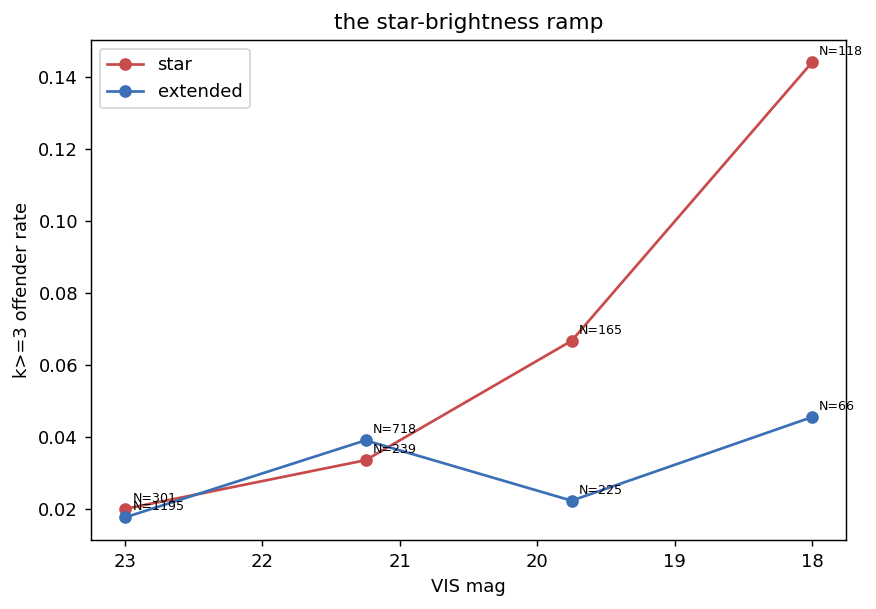
\includegraphics[width=\textwidth]{nb23_star_brightness_ramp.png}
    \column{0.48\textwidth}
      Offender rate (\alert{v10 production head}) for stars ramps 2\% $\to$ \alert{14\%} from VIS 24 to VIS 17; extended sources stay flat.
      \vspace{0.3em}

      {\footnotesize Population: the 3{,}185 sources with $\geq2$ bright (S/N$>$20) Rubin bands, the only ones the $k$ statistic can score, out of 37{,}796 in the catalog; N labels are the per-bin denominators of that eligible population, and rate $\times$ N summed over bins and classes recovers the 113.}
      \vspace{0.6em}

      Further mechanisms tested and \alert{ruled out} (beyond the WCS and proper motion of the previous slide):
      {\footnotesize
      \begin{itemize}
        \item tile-edge context (paired same-source test: $+0.1$\mas)
        \item companions within $2''$ (13\% vs 20\% control)
        \item VIS saturation (onset $\approx$17, masked not clipped; offender cores pristine)
      \end{itemize}}
  \end{columns}
\end{frame}

% --------------------------------------------------------------
\begin{frame}{Gaia adjudicates: the head is wrong, the labels are fine}
  \begin{columns}
    \column{0.52\textwidth}
      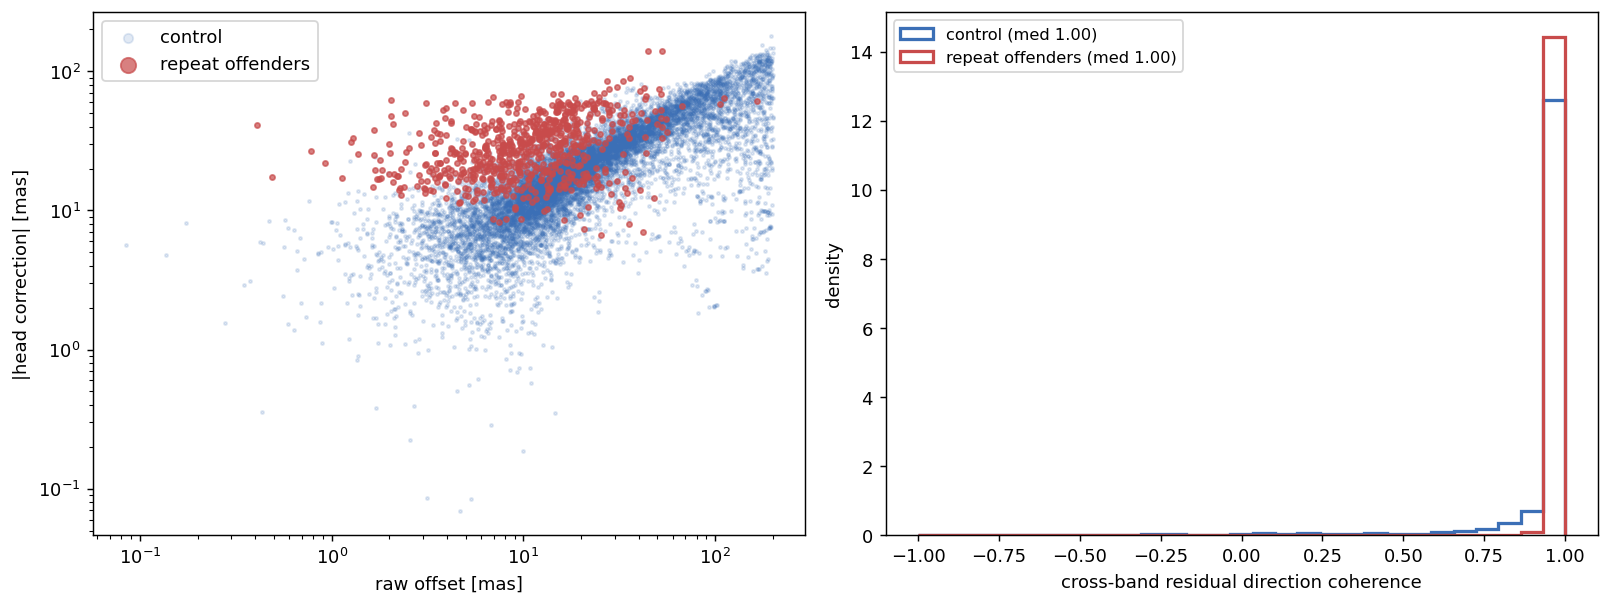
\includegraphics[width=\textwidth]{nb23_offender_mechanism.png}
    \column{0.46\textwidth}
      Against PM-propagated Gaia DR3 (epoch 2024.83), per star:
      \vspace{0.4em}
      \begin{center}
      \begin{tabular}{lcc}
        \toprule
        & VIS label & head (v10) \\
        \midrule
        offender stars ($k\geq3$) & \alert{7.0\mas} & 22.9\mas \\
        all Gaia stars & 9.5\mas & 12.2\mas \\
        \bottomrule
      \end{tabular}
      \end{center}
      \vspace{0.5em}
      Left: offenders receive corrections \alert{larger than the raw disagreement} ($|c|\!\sim\!28$\mas{} vs raw $\sim$11\mas), coherently in every band: the head asserts a center the classical centroids contradict.
      \vspace{0.4em}

      Reading (as of July): a brightness-dependent divergence between the Gaussian-fit convention and the head's feature-encoded center. \textit{The actual mechanism was found in August --- slides ahead.}
  \end{columns}
\end{frame}

% --------------------------------------------------------------
\begin{frame}{The cure: route by uncertainty, do not gate by magnitude}
  \supersededbanner
  \begin{columns}
    \column{0.46\textwidth}
      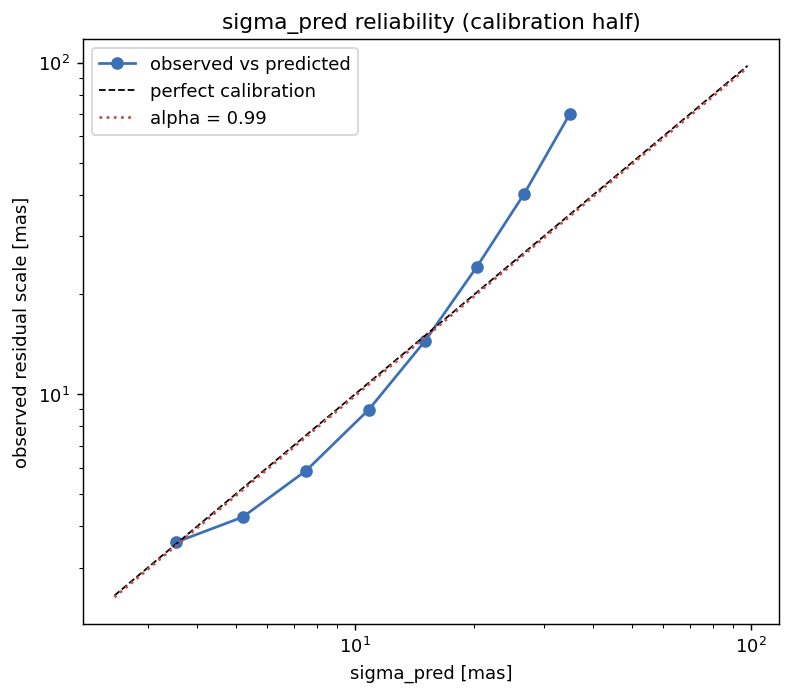
\includegraphics[width=\textwidth]{nb24_sigma_reliability.png}
    \column{0.52\textwidth}
      Two estimators of the same VIS-convention position: classical (error scale $\sigma_{\rm cl}$ from S/N and class) and head-corrected (the head's own $\sigma_{\rm pred}$).
      \vspace{0.4em}
      \begin{equation*}
        \mathrm{combined} = (1-w)\,\mathrm{raw} + w\,\mathrm{resid},
      \end{equation*}
      \begin{equation*}
        w = \frac{\sigma_{\rm cl}^2 - \rho\,\sigma_{\rm cl}\sigma_h}{\sigma_{\rm cl}^2 + \sigma_h^2 - 2\rho\,\sigma_{\rm cl}\sigma_h}
      \end{equation*}
      \begin{itemize}
        \item $\sigma_{\rm pred}$ is nearly perfectly calibrated in bulk ($\alpha=0.99$); the over-confidence lives only in the offender tail.
        \item The correlation matters: head and classical errors share photons ($\rho\approx0.8$ extended, $0.5$ stars); naive inverse variance costs 2\mas{} at the faint end, the correlation-aware weight costs nothing.
        \item All calibrations fit on half the tiles; all results from the other half.
      \end{itemize}
  \end{columns}
\end{frame}

% --------------------------------------------------------------
\begin{frame}{Where the weight moves: the two error bars, side by side}
  \supersededbanner
  \begin{center}
    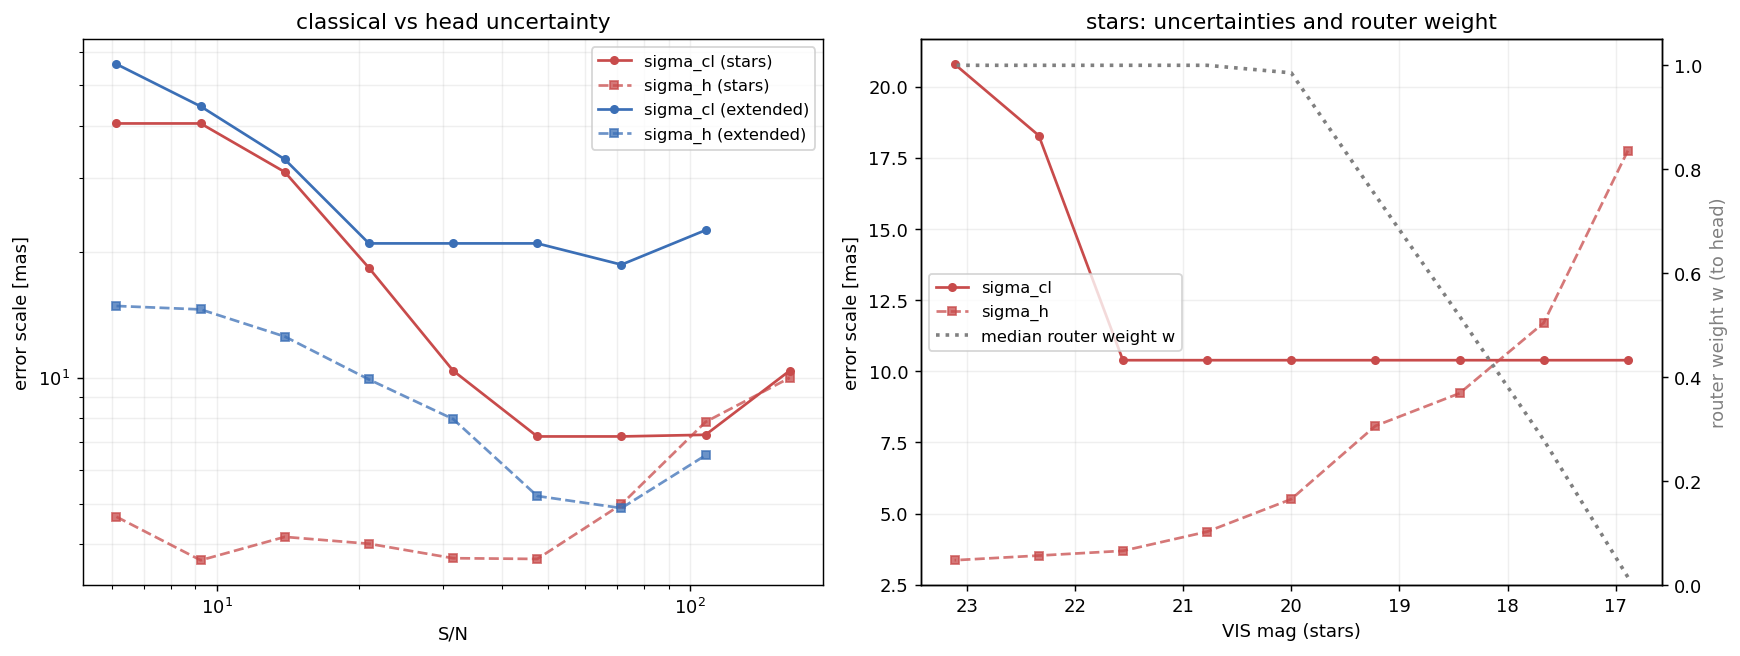
\includegraphics[width=0.80\textwidth]{nb24_sigma_cl_vs_h.png}
  \end{center}
  \vspace{-0.5em}
  {\small
  \begin{itemize}
    \item Extended sources: classical centroiding is morphology limited ($\sigma_{\rm cl}\gtrsim20$\mas{} at every S/N); the curves \alert{never cross}, so galaxies are pure head.
    \item Stars: crossing at S/N $\approx$ 108 (VIS $\approx$ 18.2); the weight (gray) slides 1 $\to$ 0 across VIS 20 $\to$ 17. The magnitude gate is \alert{derived from the uncertainties}, not imposed.
    \item $\sigma_h$ \alert{rises} for bright stars: the uncertainty channel partially knows the head struggles there; the offenders are the tail where that self-awareness fails.
  \end{itemize}}
\end{frame}

% --------------------------------------------------------------
\begin{frame}{Result: best of both estimators, everywhere}
  \supersededbanner
  \begin{center}
    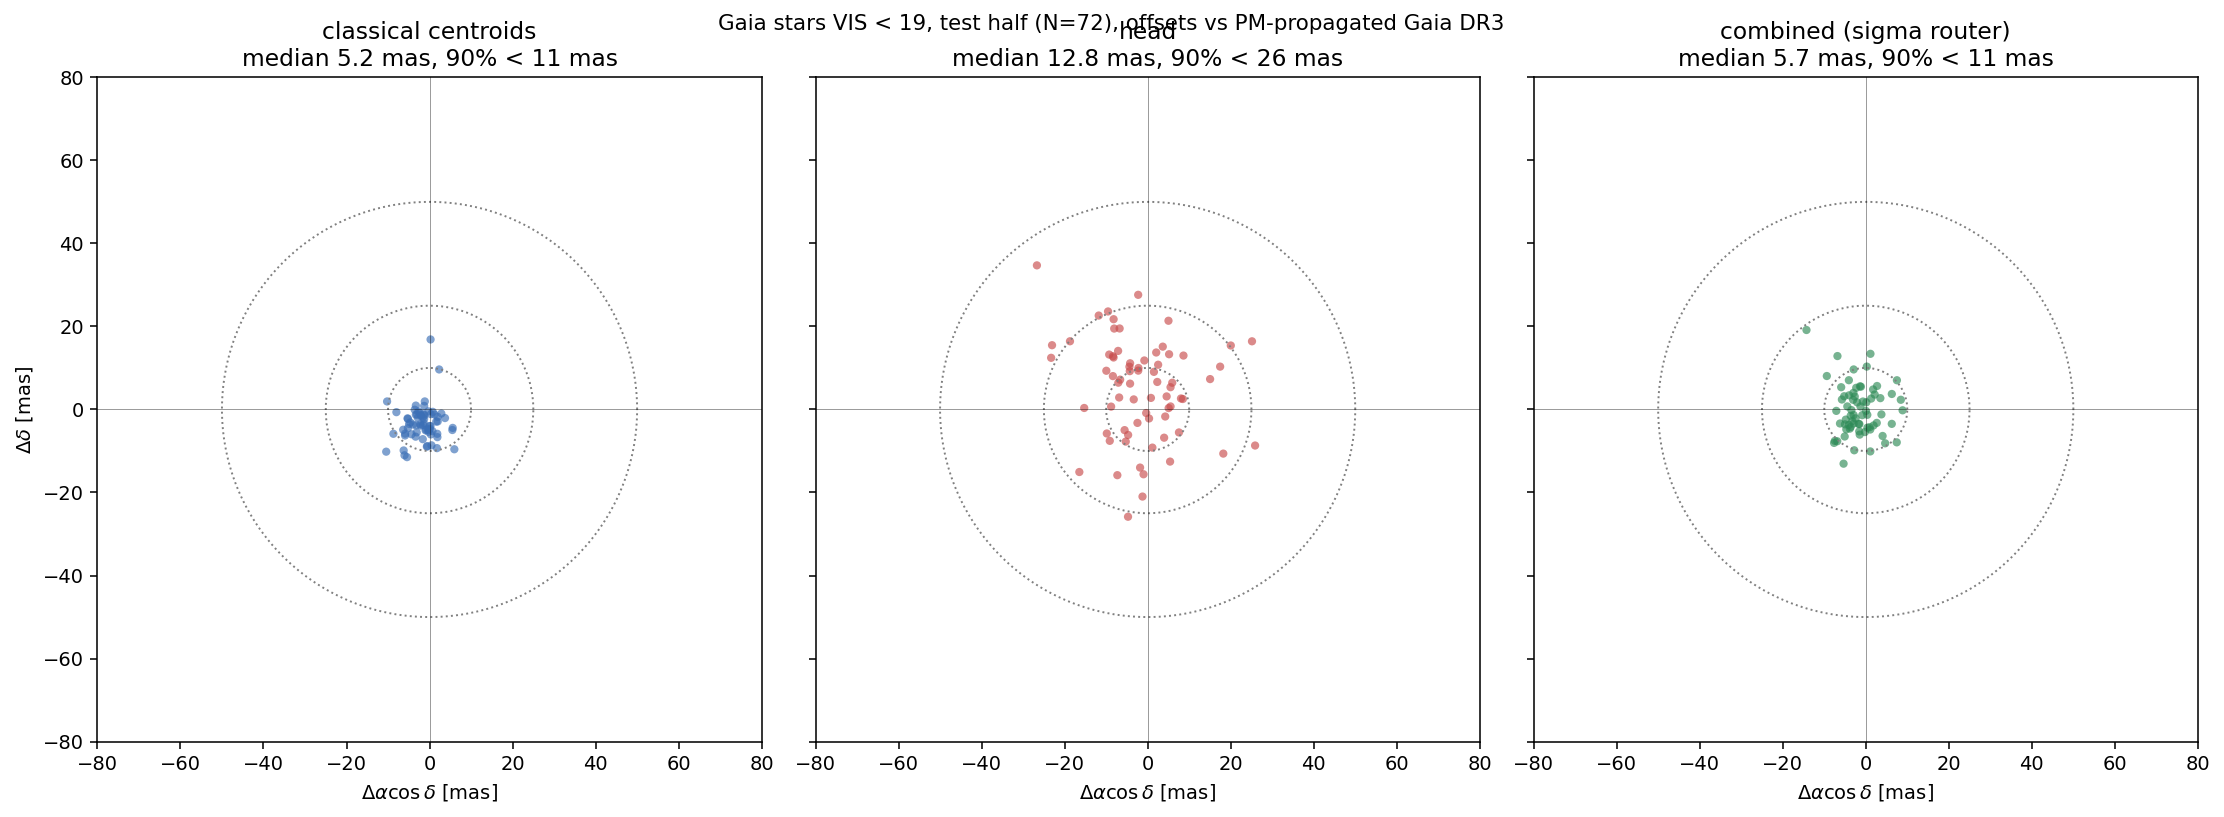
\includegraphics[width=0.92\textwidth]{nb24_gaia_circles_router.png}
  \end{center}
  \vspace{-0.3em}
  \begin{center}
  \begin{tabular}{lccc}
    \toprule
    median radial offset [mas] & classical & head & router \\
    \midrule
    all sources & 50.6 & 14.6 & \alert{14.7} \\
    bright stars, vs Gaia truth & \alert{5.2} & 12.8 & \alert{5.4} \\
    faint (S/N $<$ 10) & 64.9 & 18.5 & \alert{18.5} \\
    \bottomrule
  \end{tabular}
  \end{center}
  \vspace{0.3em}
  Bright stars made worse than classical: 38\% (head) $\to$ 16\% (router), with the large-amplitude halo gone.
\end{frame}

% --------------------------------------------------------------
\begin{frame}{The concordance field does not care, and one real discovery}
  \begin{columns}
    \column{0.44\textwidth}
      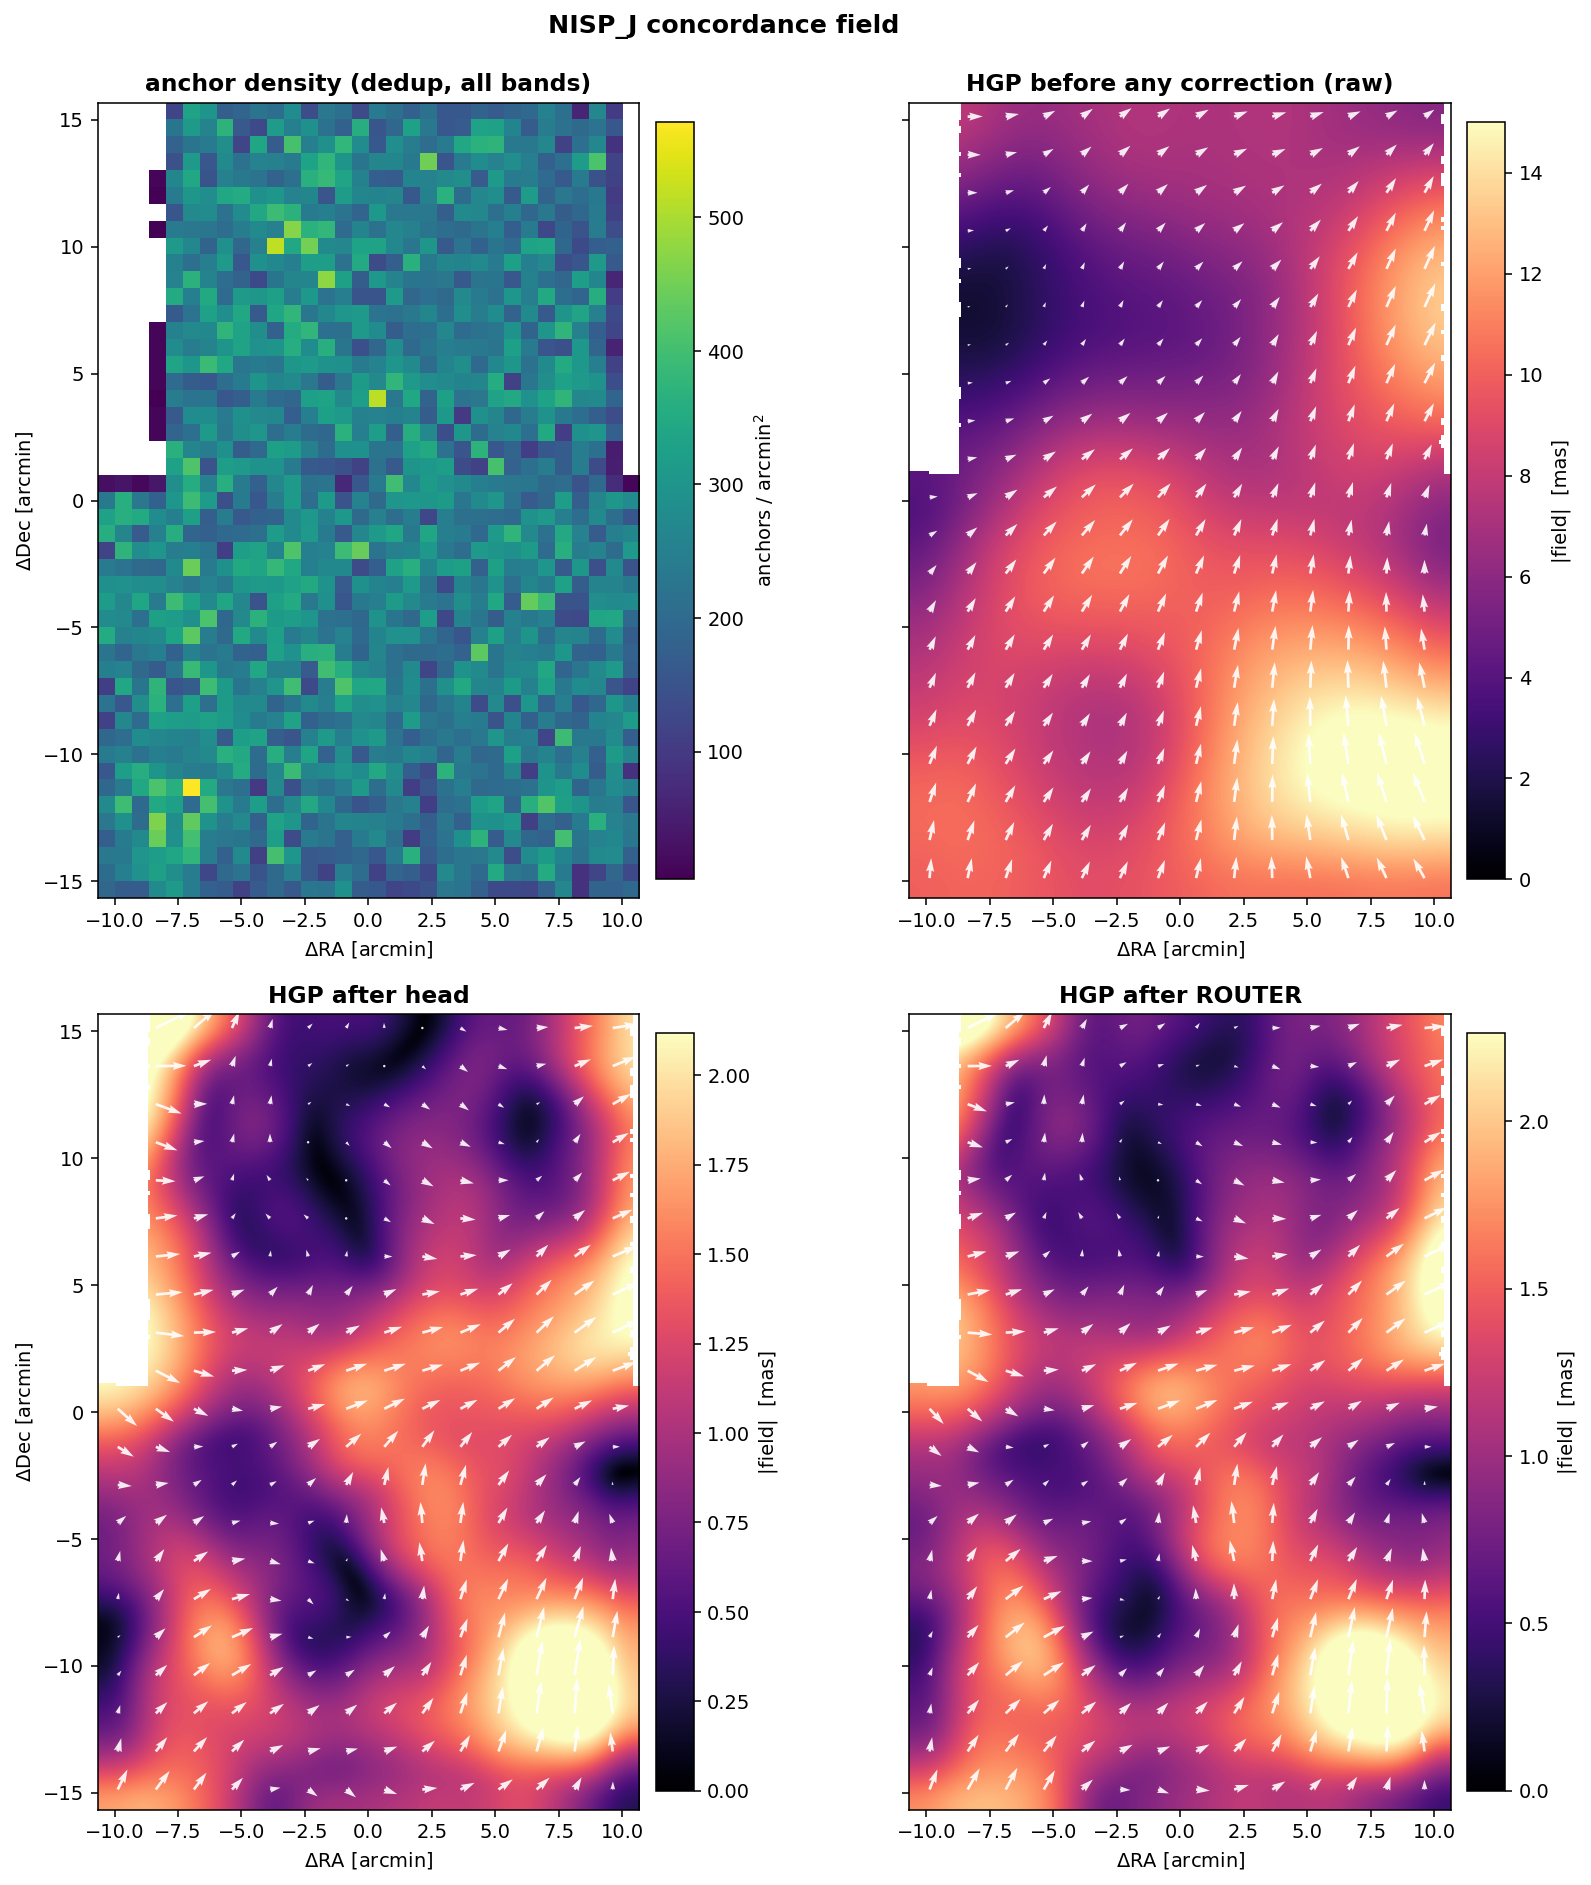
\includegraphics[width=\textwidth]{nb24_field_hgp_raw_head_router.png}
    \column{0.54\textwidth}
      \begin{itemize}
        \item Refit the field (HGP super-tight, PINN) on router residuals (v10-era archives): median change \alert{0.16\mas}, an order of magnitude below the field amplitude. The robust fit had already absorbed the 113 outliers; Figure 10 and the FITS products stand.
        \item The $\sim$15\mas{} lobe at lower right is \alert{real}: coherent in 8 of 9 bands relative to VIS, normal anchor coverage, both solvers agree, and it sits within MER tile TILE102043549. Eight rulers agree and one does not: a localized feature of the \alert{VIS solution}.
        \item By construction no VIS-trained correction can remove it; the released raw-field FITS is precisely the map that carries it.
      \end{itemize}
  \end{columns}
\end{frame}


% ==============================================================
% AUGUST 2026: THE MECHANISM, THE FIX, AND CLOSURE (v11)
% ==============================================================
\begin{frame}{August: the trail --- displacements follow one instrument-locked axis}
  \begin{columns}
    \column{0.46\textwidth}
      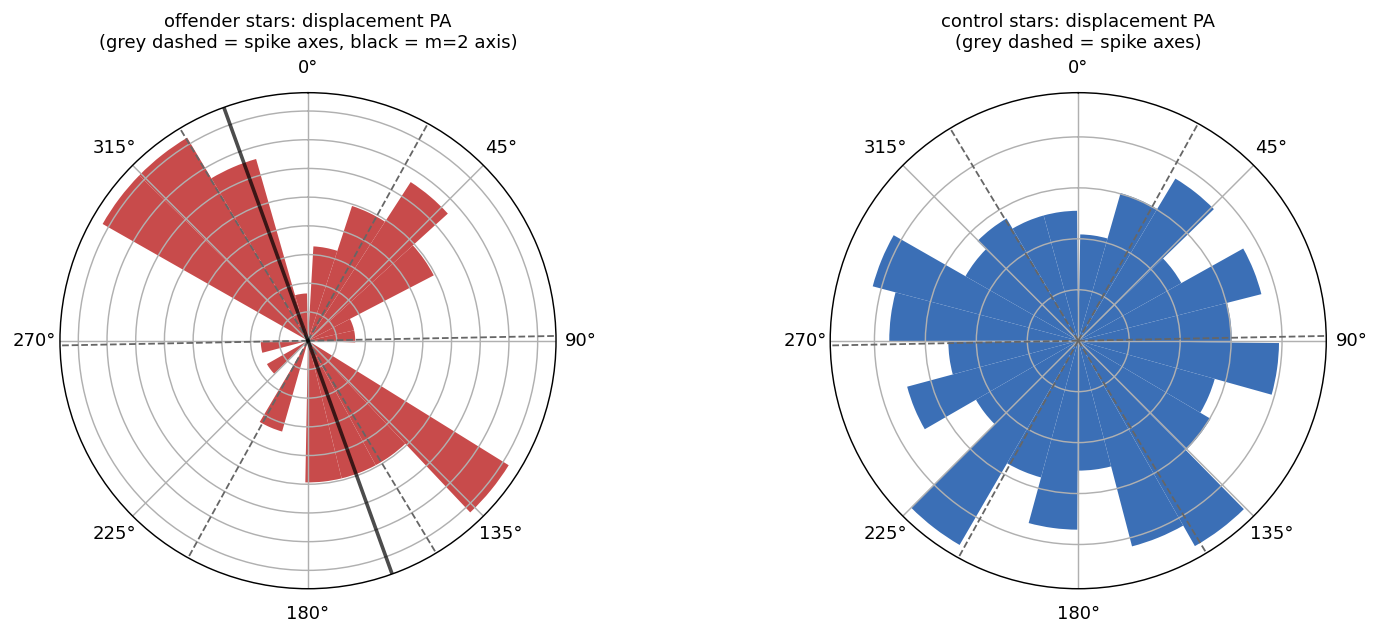
\includegraphics[width=\textwidth]{nb23_offender_directions.png}\\{\scriptsize v10 archive (ECDFS)}
    \column{0.52\textwidth}
      \begin{itemize}
        \item Offender displacements are \alert{elongated along a single sky axis} (PA $\approx160^\circ$, both signs, no net direction); controls are isotropic.
        \item The axis \alert{rotates with the Euclid instrument} between ECDFS and EDF-S (spike phases $28.9^\circ\to49.7^\circ$).
        \item Published VIS geometry (strut angles + four-corner CCD readout) predicts the readout axis \alert{1.9$^\circ$} from the measured one, with zero tuned parameters --- in both fields, one parity.
        \item Yet a signed flux stack shows \alert{no trailed light} (CTI ruled out), and rotating a star's own pixels rotates its displacement: the cause lives in the images as the network sees them.
      \end{itemize}
  \end{columns}
\end{frame}

% --------------------------------------------------------------
\begin{frame}{The mechanism: a hard S/N clamp erases bright-star cores}
  \begin{center}
    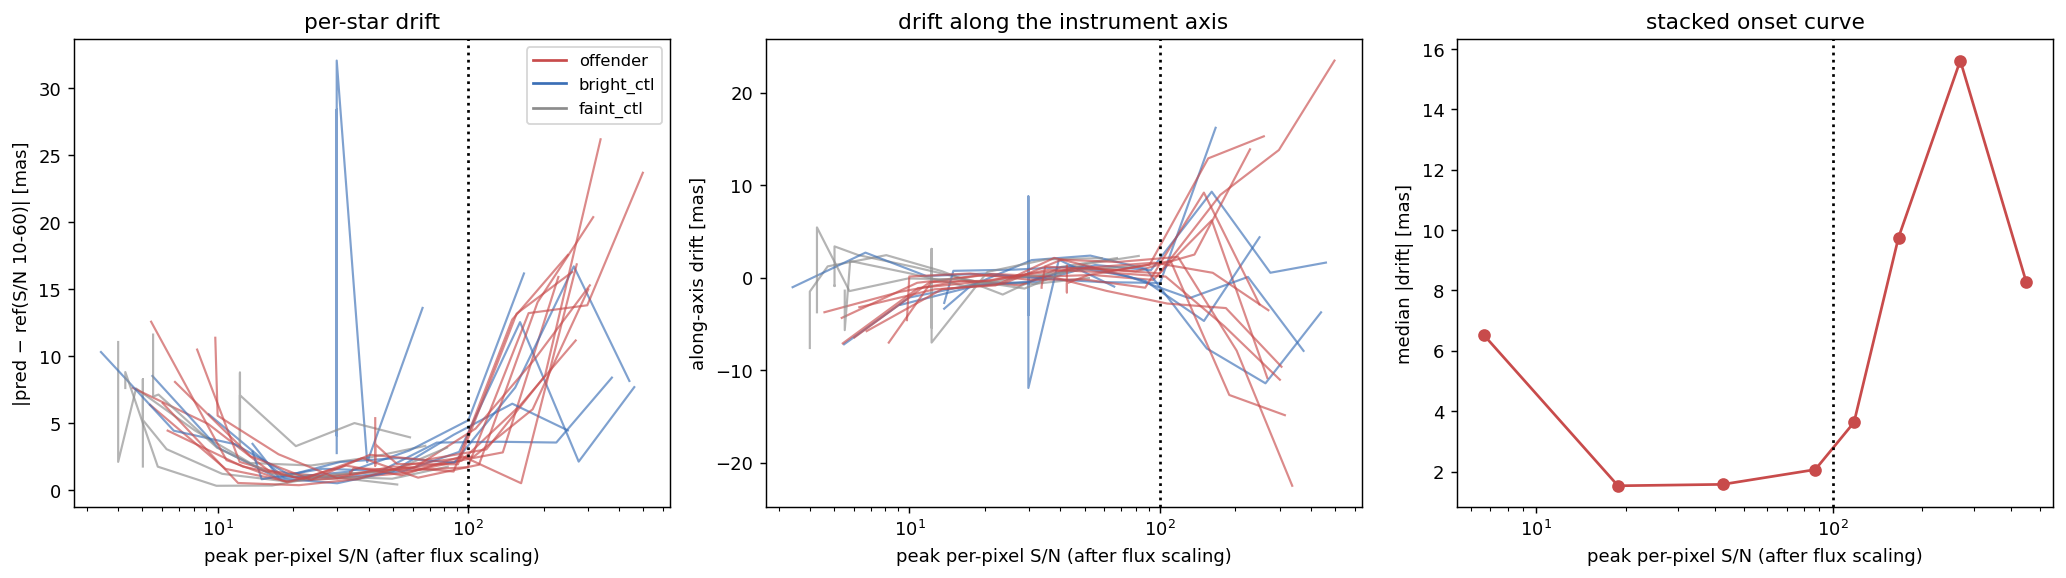
\includegraphics[width=0.95\textwidth]{nb23_clamp_onset.png}\\{\scriptsize causal interventions on the v10 production model}
  \end{center}
  \vspace{-0.4em}
  {\small
  \begin{itemize}
    \item Every input enters the foundation as \texttt{(image/rms).clamp(-10, 100)} --- unchanged since v4. Above per-pixel S/N 100 a star's core is a \alert{featureless plateau}; the reconstruction targets are clamped identically, so \alert{no loss ever saw the missing information}.
    \item Causal test: scale a real star's flux $\times$50 --- the head places the \emph{same star} to 1--2\mas{} for peak S/N 10--90, and the displacement \alert{switches on exactly above S/N $\approx$ 100} (a threshold, not a trend), reaching the archived 11--26\mas{} at native flux.
    \item Rotating the star's local image $180^\circ$ flips the displacement (median $\cos=+0.91$): each star's error is deterministic, written in its own pixels.
  \end{itemize}}
\end{frame}

% --------------------------------------------------------------
\begin{frame}{Why an axis from a scalar cut? The shape of what survives}
  \begin{center}
    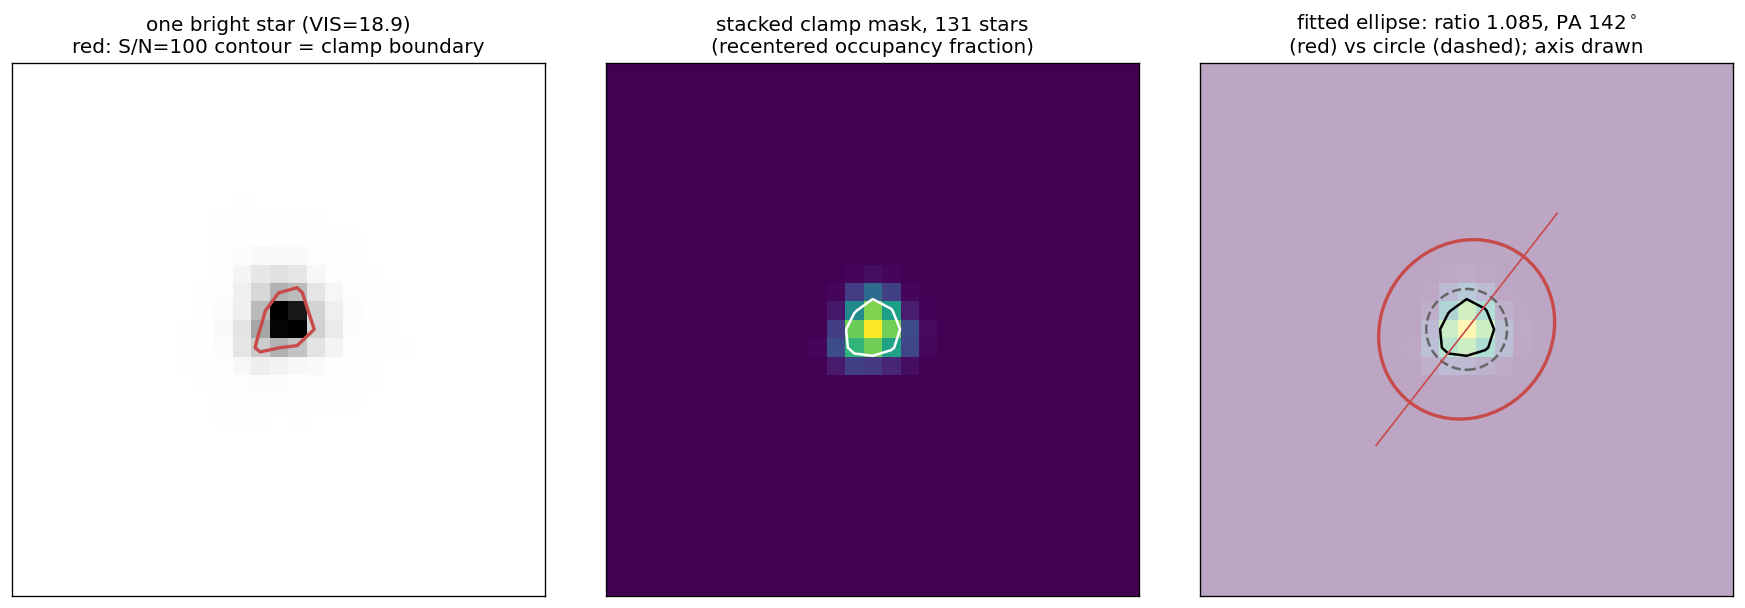
\includegraphics[width=0.92\textwidth]{clamp_mask_stack.png}
  \end{center}
  \vspace{-0.6em}
  {\footnotesize
  \begin{itemize}
    \item The clamp is isotropic, but the surviving information is not: per star the S/N=100 plateau (left, red) is a ragged blob, yet the \alert{stack of 131 masks} (middle) is measurably elliptical --- \alert{axis ratio 1.085} (CI [1.05, 1.20]), \alert{major axis PA $142^\circ\pm15^\circ$}, consistent with the offender displacement axis ($160^\circ\pm9^\circ$) and the instrument frame.
    \item An elongated boundary constrains the centroid weakly along its major axis: errors along one axis, both signs, no net drift --- the measured $m{=}2$-without-$m{=}1$ signature; the flux stack shows \alert{no trailed light} (CTI ruled out).
    \item Under v11 the same elongation is still in the images --- with the core restored, the head stops leaning on the boundary and the axis signal vanishes. {\footnotesize Per-star sign mechanism (subpixel phase?) untested.}
  \end{itemize}}
\end{frame}

% --------------------------------------------------------------
\begin{frame}{The fix is one line, then retrain: v11}
  \begin{center}
    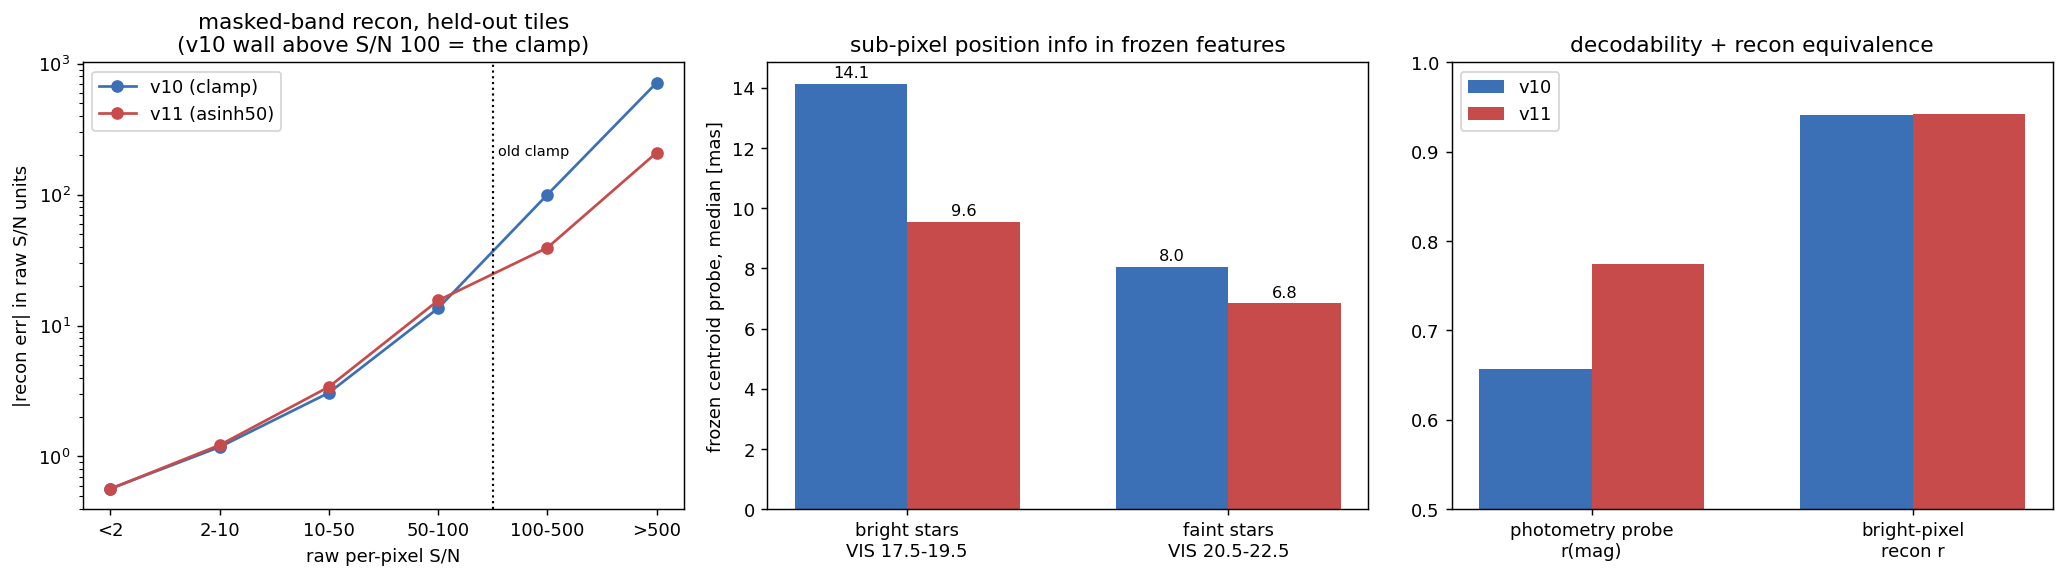
\includegraphics[width=0.95\textwidth]{nb30_v11_gate.png}
  \end{center}
  \vspace{-0.4em}
  {\small
  \begin{itemize}
    \item \texttt{clamp(-10,100)} $\to$ \texttt{50*asinh(x/50)} in stems \emph{and} reconstruction targets; foundation retrained from scratch, identical recipe (\texttt{jaisp\_v11\_q1\_soft}).
    \item Gate: reconstruction parity in bulk (bright-pixel $r$ 0.9412 vs 0.9419); the v10 error \alert{wall above S/N 100} is gone (left); frozen centroid probe on bright stars \alert{14.1 $\to$ 9.6\mas} (middle); photometry decodability up.
    \item The position head is retrained \alert{unchanged} --- no side-channel, no reweighting. The architecture was never the problem; its inputs were.
  \end{itemize}}
\end{frame}

% --------------------------------------------------------------
\begin{frame}{Closure: the census rerun --- v10 and v11 side by side}
  \begin{center}
    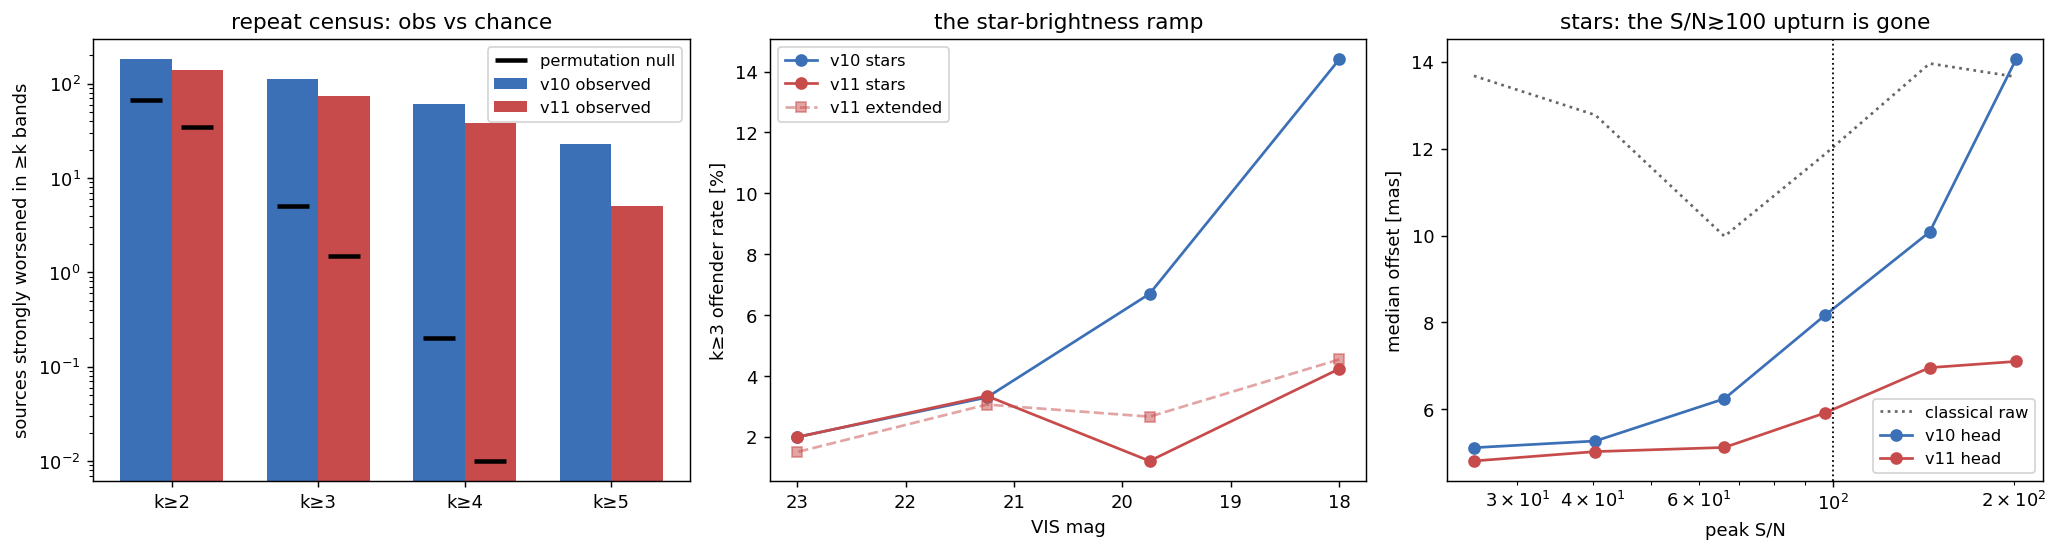
\includegraphics[width=\textwidth]{nb23_v11_closure.png}
  \end{center}
  \vspace{-0.4em}
  {\small
  \begin{itemize}
    \item The star--brightness ramp is \alert{flat} (2--4\% at all magnitudes, indistinguishable from galaxies; was 2 $\to$ 14.4\%).
    \item The S/N $\gtrsim$ 100 upturn is \alert{reversed}: the v11 head sits at 5--7\mas{} where classical raw is 10--14 --- it now adds value on bright stars. General Gaia stars: head at label parity (10.8 vs 9.5\mas).
    \item Faint-end headline untouched (raw 47.9 $\to$ 13.3\mas, 91\% improved --- identical to v10). Under v11 the router no longer improves any regime: the interim mitigation is \alert{retired by the cure}.
  \end{itemize}}
\end{frame}

% --------------------------------------------------------------
\begin{frame}{The original mystery is closed --- and it was hiding a smaller one}
  \small
  \textbf{Decomposition of the 113 repeat offenders:}
  \begin{center}
  \begin{tabular}{lll}
    \toprule
    $\sim$46 clamp-driven bright stars & \alert{cured by v11} & (the ramp, the upturn, the axis) \\
    $\sim$67 source-specific cases & \alert{survive both foundations} & (the new open question) \\
    \bottomrule
  \end{tabular}
  \end{center}
  \vspace{0.4em}
  The survivors: the \emph{same sources} under two independently trained foundations, same signature (raw $\sim$10\mas, coherent $\sim$30\mas{} head displacement; Gaia still against the head, 29.5 vs 9.6\mas{} for the 8 Gaia stars among them). Not brightness-selected, not resolved blends (12\% vs 20\% control), not extended.
  \vspace{0.4em}
  \begin{itemize}
    \item Cause is outside the foundation: in the data or labels of these specific sources, or in what both trainings share (label pipeline, tiles). Suspects: \alert{sub-arcsecond pairs below MER's deblending limit}; convention-ambiguous profiles with unstable training labels.
    \item 0.2\% of the catalog; the uncertainty router covered them in the meantime. \alert{Resolved in September --- next slides.}
  \end{itemize}
\end{frame}

% ==============================================================
% SEPTEMBER 2026: THE SURVIVORS ARE A GALAXY POPULATION; THE ANCHORED HEAD
% ==============================================================
\begin{frame}{September: the survivors are a real population --- and it was there in v10 too}
  \begin{columns}
    \column{0.50\textwidth}
      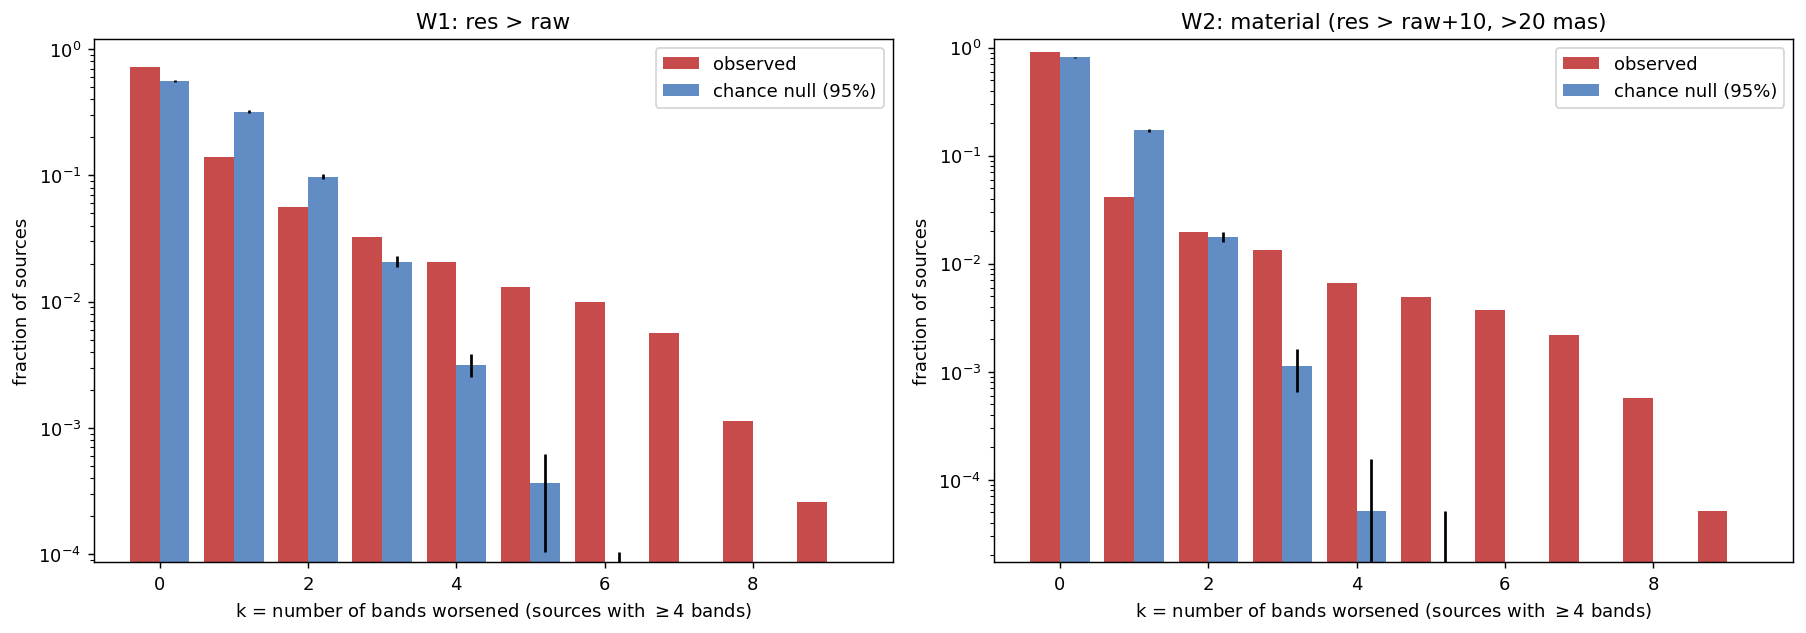
\includegraphics[width=\textwidth]{nb31_coherence_null.png}\\{\scriptsize v11 plain head, 790 tiles, 37.9k sources (io/31)}
    \column{0.48\textwidth}
      {\footnotesize
      \begin{itemize}
        \item Count in how many bands a source is \emph{materially} worsened (res $>$ raw$+10$\mas{} and $>20$\mas). The $k\le2$ bins match the chance null built from empirical per-(band, S/N) rates: the bulk of the 8.9\% worsened measurements is luck.
        \item At $k\ge3$: \alert{604 sources (1.6\%) vs $23\pm5$ by chance} ($\times26$; $\times400$ at $k\ge4$). Within a source the residual vector points the same way in every band (median pairwise $\cos=0.997$): one deterministic wrong position per source.
        \item Isotropic across sources, no tile clustering, no sky pattern: nothing instrumental survives in v11. The cause lives in each source's own pixels.
        \item Rerun on v10: \alert{622 sources, 80\% the same objects}. Hidden at S/N $\approx13$, where one worsened band looks like chance; the bright-tail selection of July was dominated by the clamp instead.
      \end{itemize}}
  \end{columns}
\end{frame}

% --------------------------------------------------------------
\begin{frame}{Who they are: extended galaxies, where the head is precise but biased}
  \begin{columns}
    \column{0.50\textwidth}
      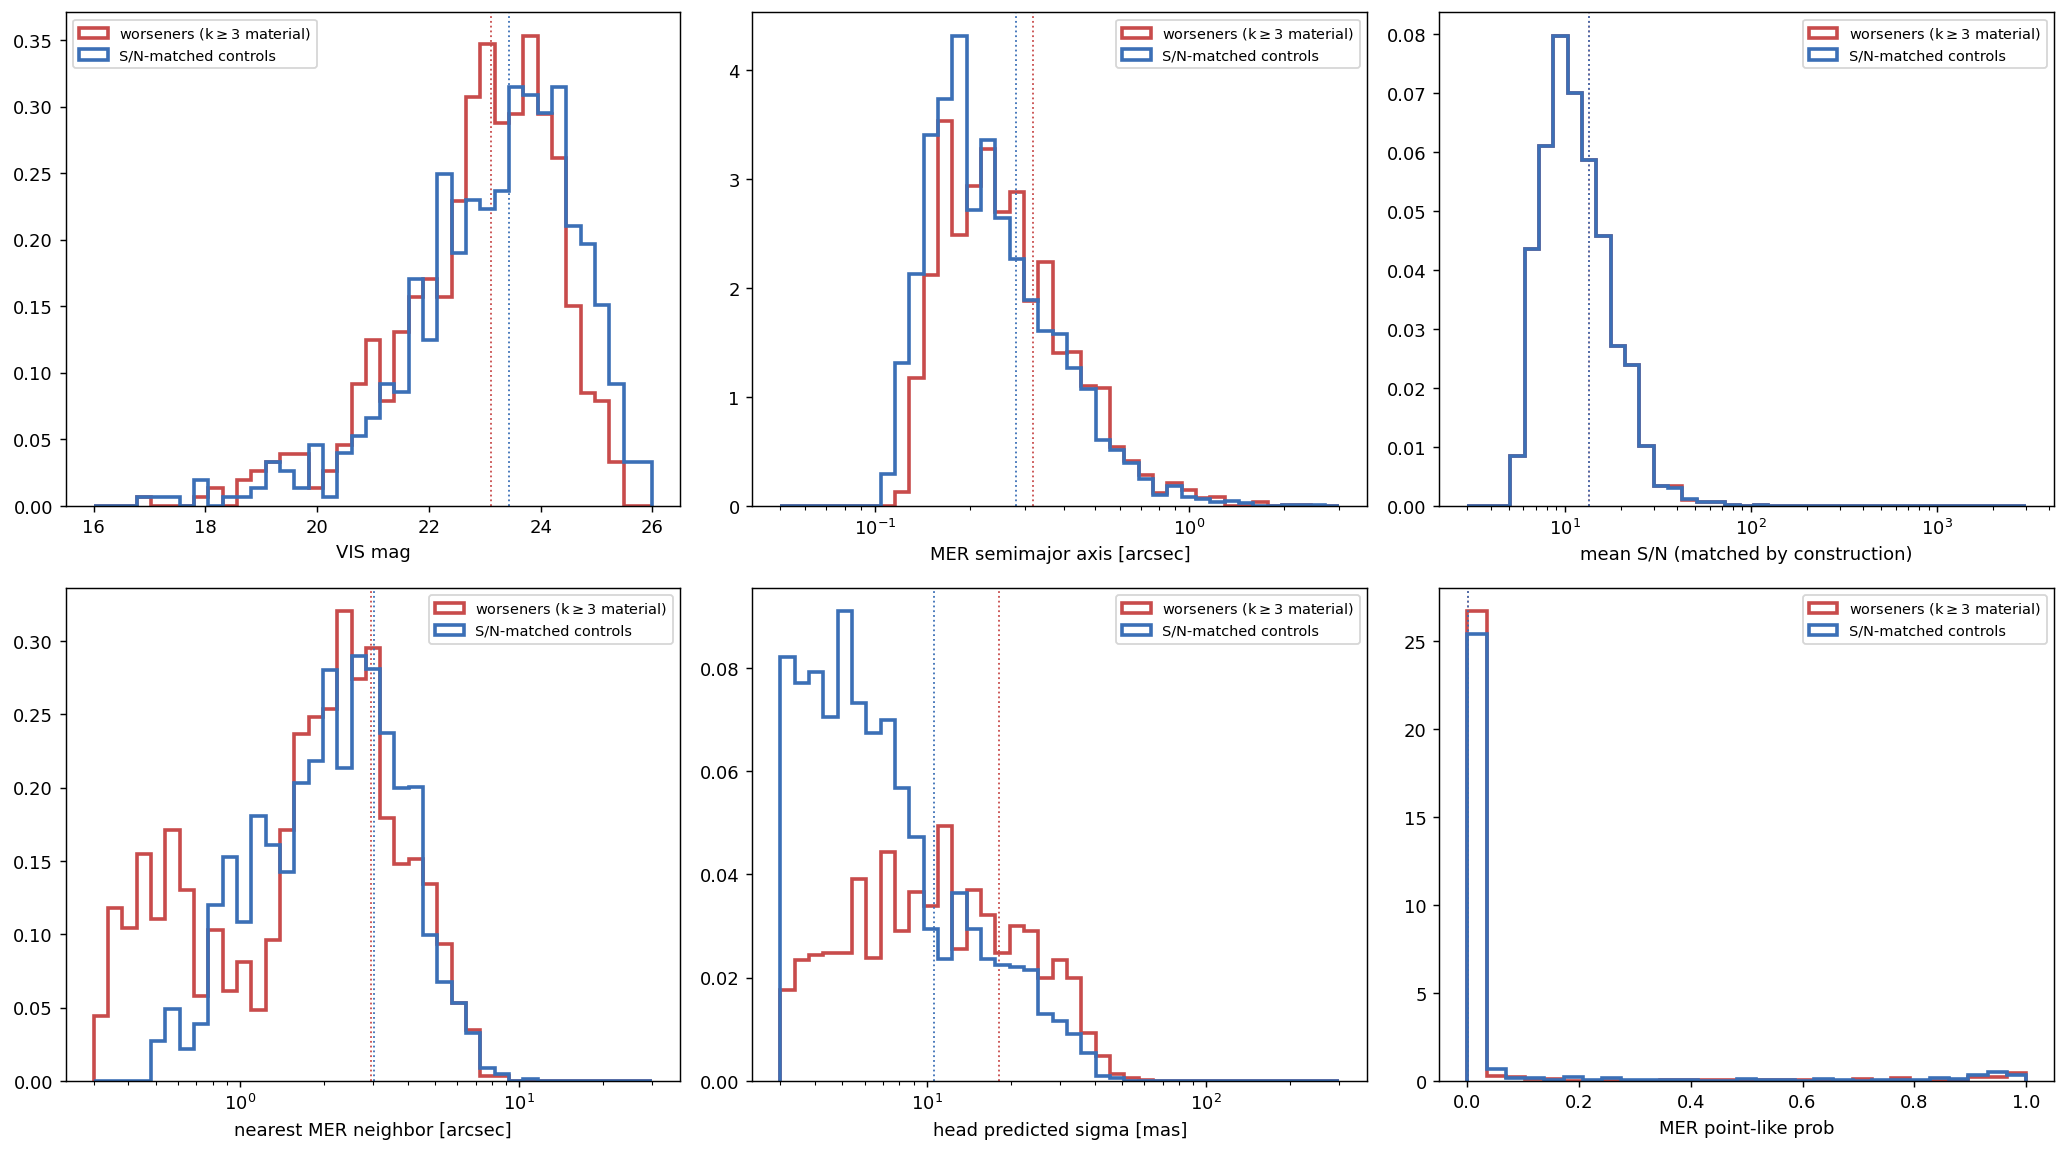
\includegraphics[width=\textwidth]{nb31_population_props.png}
    \column{0.48\textwidth}
      {\footnotesize
      \begin{itemize}
        \item vs S/N-matched controls: galaxies in both (point-like 1\%), but \alert{brighter (VIS 23.1 vs 23.4) and larger (0.32$''$ vs 0.28$''$)} at the same S/N; $\times1.7$ excess of sub-arcsecond MER companions (7.6\% vs 4.5\% within $1''$). The head's own $\sigma$ is elevated (18 vs 11\mas): it partially knows.
        \item Against the VIS light itself (peak, and $0.75''$ flux centroid): the head sits \alert{2--2.6$\times$ farther than the label} on worseners, isolated and paired alike (50 vs 23\mas{} to the peak); on controls head and label are equivalent. Band-to-band the head is the tighter estimator everywhere (13 vs 31\mas{} RMS).
        \item Reading: \alert{precise but biased} --- one reproducible $\sim$40\mas{} offset per source matching no natural photometric center; on chromatic sources it lies along the color axis, toward the blue/clumpy light. The \alert{tight core of 315 sources (0.8\%)}, 89\% persistent across v10/v11, is the true model-bias population.
      \end{itemize}}
  \end{columns}
\end{frame}

% --------------------------------------------------------------
\begin{frame}{Fix candidates: loss-based fixes fail, the anchored head wins}
  \begin{center}
    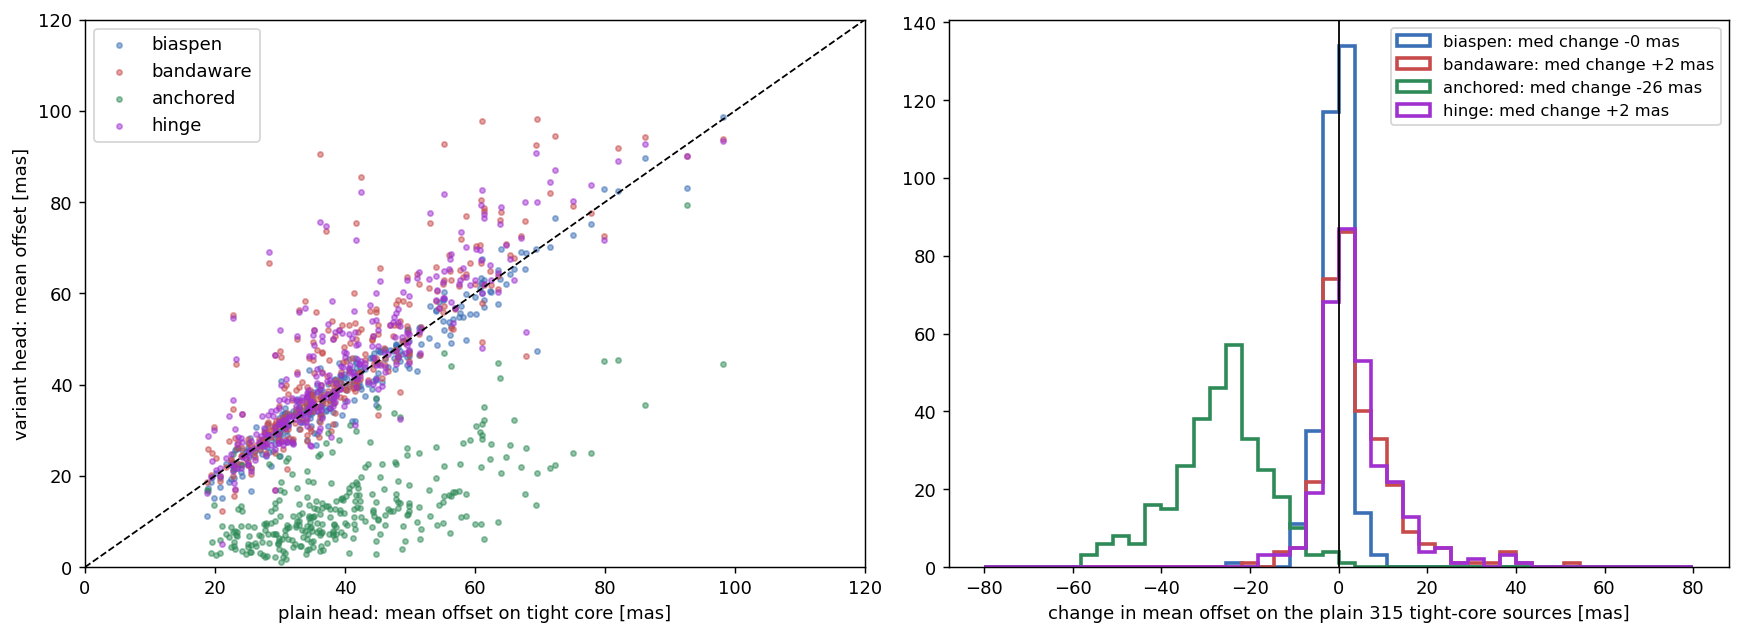
\includegraphics[width=0.50\textwidth]{nb31_fix_verdict.png}
  \end{center}
  \vspace{-1.0em}
  {\footnotesize
  \begin{center}
  \begin{tabular}{lcccccc}
    \toprule
    head & overall med & faint med & coherent ($k\ge3$, null) & tight core & $\cap$ plain 315 & control RMS \\
    \midrule
    plain      & 14.4 & 18.8 & 604 (22) & 315 & ---  & 9.9 \\
    biaspen (loss)    & 15.1 & 19.7 & 542 (18) & 297 & 260 & 10.5 \\
    bandaware (arch.) & 9.7  & 10.9 & 1113 (89) & 662 & 283 & 6.8 \\
    hinge (loss)      & 9.6  & 10.8 & 1061 (82) & 639 & 282 & 6.9 \\
    \textbf{anchored} & \textbf{7.2} & \textbf{8.6} & \textbf{235 (2)} & \textbf{37} & \textbf{6} & 7.7 \\
    \bottomrule
  \end{tabular}
  \end{center}
  \begin{itemize}
    \item Identical rows scored for every head, no worsener ever a training signal (medians in mas). \alert{Anchored:} an iterated Gaussian-weighted VIS centroid computed in the forward pass, with its photon-noise $\sigma$; the network adds only a residual bounded at a few$\times$ that noise. Tight core \alert{315 $\to$ 37 (6 of the original survive)}, every global metric better at once. Three loss-based fixes failed (NLL, biaspen, hinge): the failure is representational, not an optimization artifact.
  \end{itemize}}
\end{frame}

% --------------------------------------------------------------
\begin{frame}{The anchored head: gains are global, not tail surgery}
  \begin{center}
    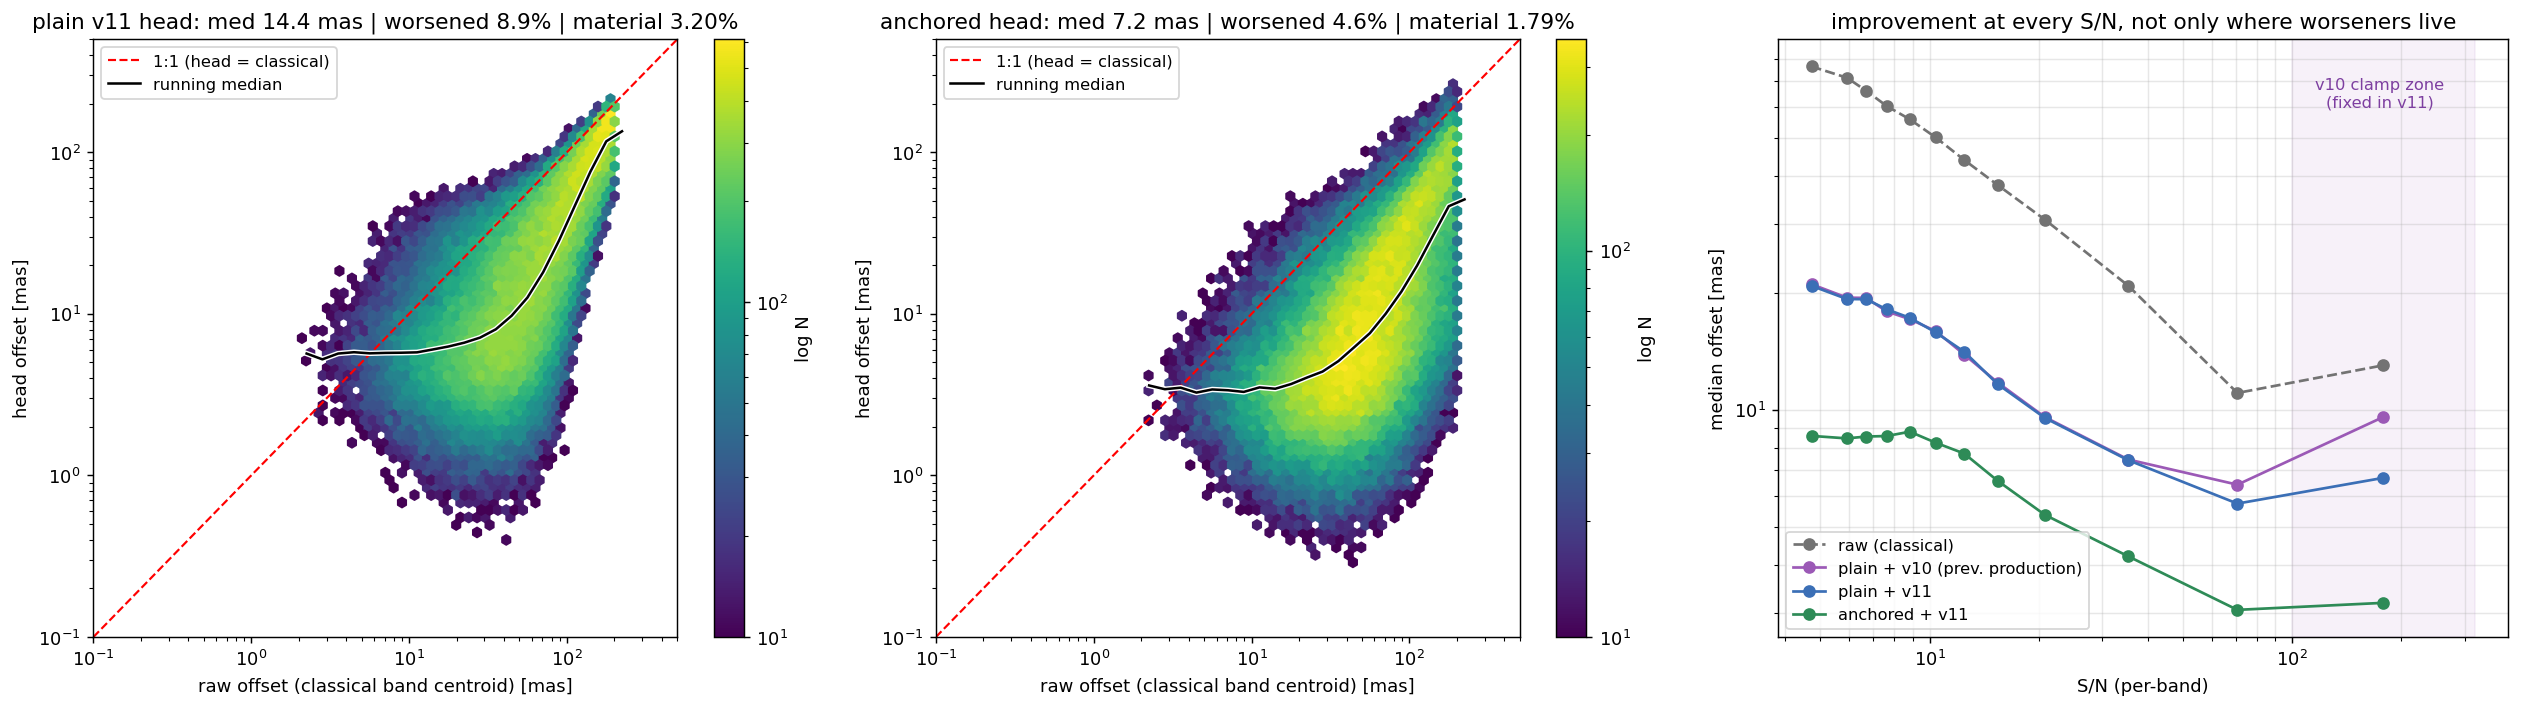
\includegraphics[width=0.88\textwidth]{nb31_full_population_plain_vs_anchored.png}
  \end{center}
  \vspace{-0.6em}
  {\footnotesize
  \begin{itemize}
    \item Anchored sits below plain at \alert{every} raw offset and every quantile: p50 \alert{14.4 $\to$ 7.2}\mas, p90 79 $\to$ 45, faint tercile 19.7 $\to$ 8.5, bright 9.4 $\to$ 5.3. Worsened fraction 8.9 $\to$ 4.6\% (material 3.2 $\to$ 1.8\%); improves on raw for 95.4\% of measurements.
    \item The faint end, where no worsener was ever flagged, improves the most: there the bound is open and the learned residual does the work. On bright stars the anchor pins the head to the classical floor.
    \item Right: the v10 upturn above S/N 100 (clamp) vs v11; the anchored gain on top is head design, not foundation version.
    \item Adoption gates passed (2026-08-31): \alert{EDF-S with no retraining} median 6.4\mas{} (plain 13.9); \alert{patch-disjoint} retrain 6.9\mas{} vs 9.2 random-split --- no overlap leakage. Adopted as production 2026-09-01; retrained on v11 detector labels 2026-09-06 (\texttt{latent\_position\_v11\_anchored\_v11labels}), the archive behind paper Figs.\ 7, 8, 11.
  \end{itemize}}
\end{frame}

% --------------------------------------------------------------
\begin{frame}{The external ruler and the error bars: Gaia recheck and $\sigma$ calibration}
  \begin{columns}
    \column{0.56\textwidth}
      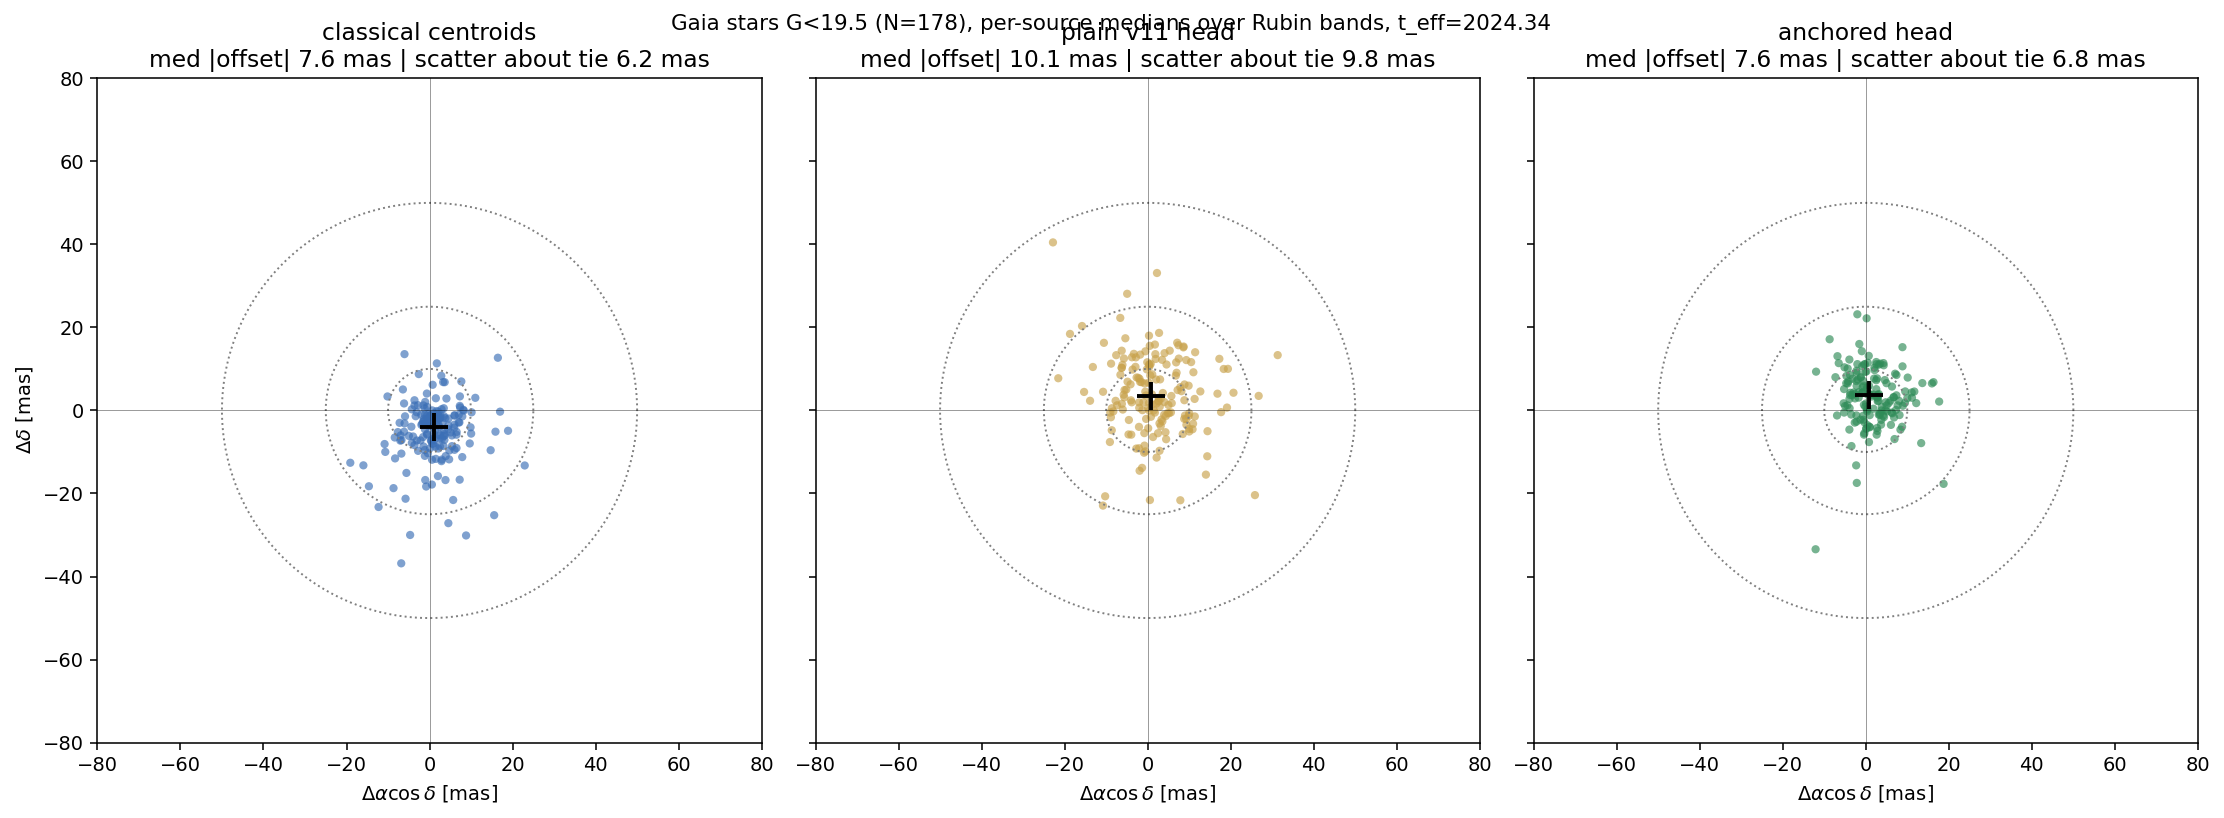
\includegraphics[width=\textwidth]{nb32_gaia_three_estimators.png}
    \column{0.42\textwidth}
      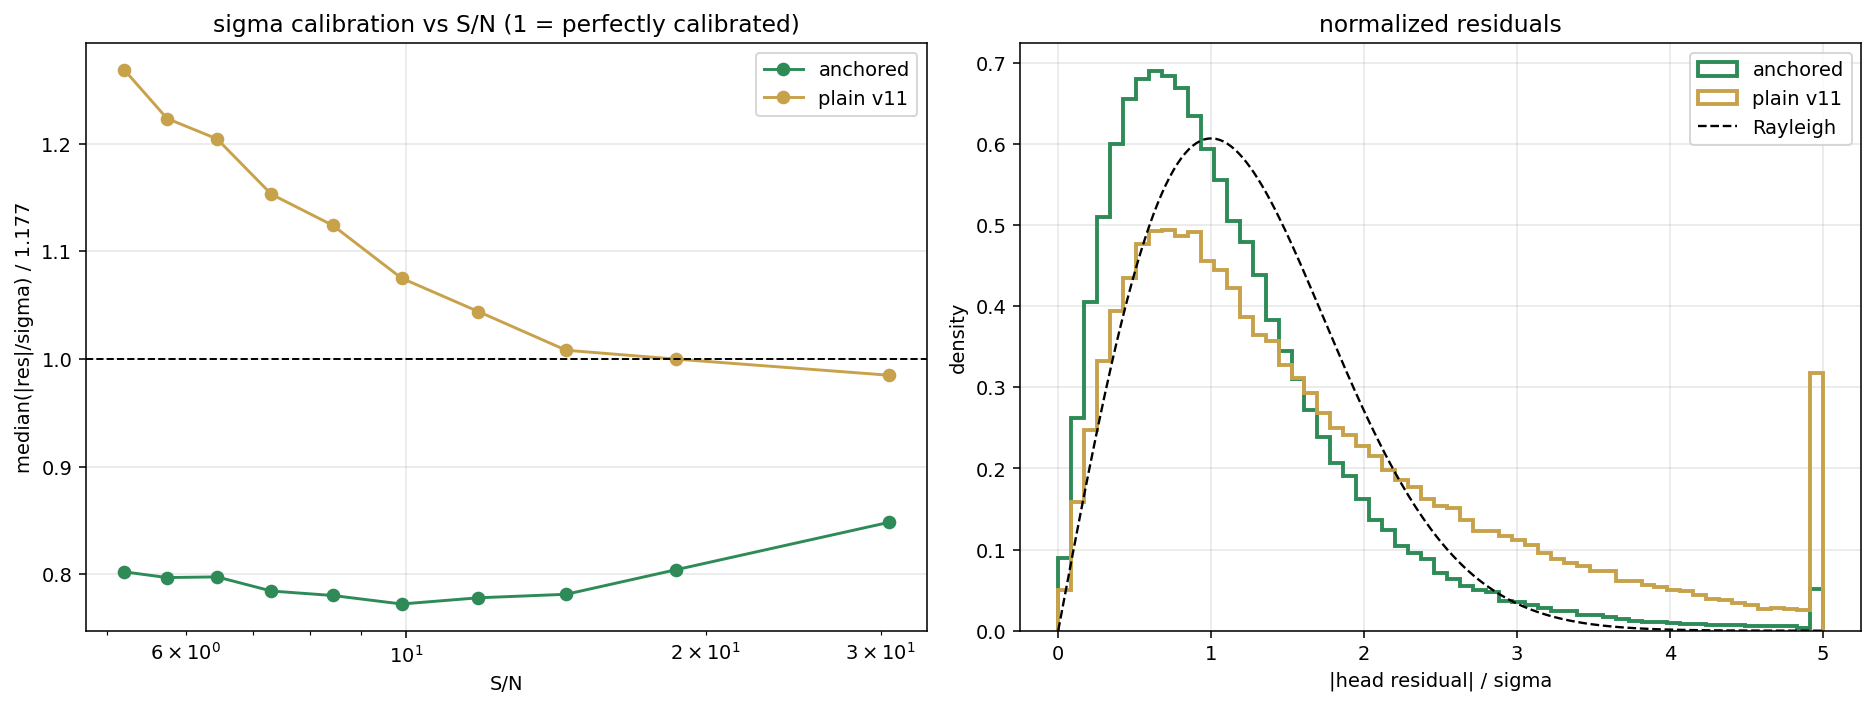
\includegraphics[width=\textwidth]{nb32_sigma_calibration.png}
  \end{columns}
  \vspace{-0.2em}
  {\small
  \begin{itemize}
    \item Gaia DR3, PM-propagated; the Q1 coadds' effective epoch re-derived as \alert{$t_{\rm eff}=2024.34$} by all three estimators (the 2024.83 value belonged to the older coadds).
    \item Bright stars ($G<19.5$): \alert{anchored = classical}, 7.6\mas{} median offset for both, scatter about the tie 6.8 vs 6.2. The plain head pays a visible Gaia penalty (10.1 / 9.8): its convention bias is real to an external ruler. Amortization now costs nothing on stars.
    \item The 7.8\mas{} Dec split between the classical tie ($-4.1$) and the head tie ($+3.7$) is the concordance field (common component 6.9\mas), not a pathology: classical Rubin centroids live in the Rubin frame, the heads in the VIS convention, Gaia sits between.
    \item $\sigma_{\rm pred}$: anchored is \alert{uniformly conservative, factor 0.79 flat in S/N} --- one global rescale calibrates it (90\% coverage 91\%). Plain $\sigma$ was miscalibrated in shape with a heavy tail (90\% coverage 74\%). The router has at most $\sim$0.5\mas{} left to collect: retired.
  \end{itemize}}
\end{frame}

% --------------------------------------------------------------
\begin{frame}{Takeaways}
  \small
  \begin{itemize}
    \item Above the 1:1 line sit two populations: mostly benign regression to the corrected floor, plus real failures concentrated in bright point sources --- diagnosed by \alert{repetition across bands}, not by any average metric.
    \item The mechanism was one line of preprocessing: a hard per-pixel S/N clamp that erased bright-star cores --- invisible to every loss curve because the targets were clamped too. \alert{Audit your input transforms; stratify metrics by regime.}
    \item Correlational forensics narrowed the suspects; \alert{causal interventions} (flux sweep, rotation) convicted. The fix is soft compression + retrain (v11): ramp flat, upturn reversed, faint-end headline untouched, detection deeper.
    \item The interim uncertainty router did its job and is retired by the cure. The 67 survivors were the visible tip of a \alert{1.6\% extended-galaxy population} where the learned center disagrees reproducibly with the classical convention --- present in v10 too, hidden at S/N $\approx13$, invisible to loss-based fixes.
    \item The cure for that one is architectural: the \alert{anchored head} computes the convention centroid in its forward pass and learns only a bounded residual. Tight core 315 $\to$ 37, medians halved at every S/N, Gaia parity on bright stars, calibrated $\sigma$; gates passed on EDF-S and patch-disjoint. Production since 2026-09-01.
    \item The paper sentence, updated: the head improves astrometry where classical methods are noise limited, and \alert{matches them} where they are systematics limited --- a single estimator for both regimes.
  \end{itemize}
\end{frame}

\end{document}
